\documentclass{article}
\usepackage[utf8]{inputenc}
\usepackage[fleqn]{amsmath}
\usepackage[T1]{fontenc}
\usepackage{parskip}
\usepackage{booktabs}
\usepackage{amsmath,amssymb,amsfonts}
\usepackage{natbib}
\usepackage{textcomp}
\usepackage{booktabs}
\usepackage{pgfplots}
\usepackage{pgfplotstable}
\usepackage{array}
\usepackage{bbold}
\usepackage{amssymb}
\usepackage[procnames]{listings}
\usepackage{color}
\usepackage{graphicx}

\addtolength{\oddsidemargin}{-.875in}
\addtolength{\evensidemargin}{-.875in}
\addtolength{\textwidth}{1.75in}

\addtolength{\topmargin}{-.875in}
\addtolength{\textheight}{1.75in}

\makeatletter
\newcommand{\distas}[1]{\mathbin{\overset{#1}{\kern\z@\sim}}}%
\newsavebox{\mybox}\newsavebox{\mysim}
\newcommand{\distras}[1]{%
	\savebox{\mybox}{\hbox{\kern3pt$\scriptstyle#1$\kern3pt}}%
	\savebox{\mysim}{\hbox{$\sim$}}%
	\mathbin{\overset{#1}{\kern\z@\resizebox{\wd\mybox}{\ht\mysim}{$\sim$}}}%
}
\makeatother

\title{Comparison between the optimal proposal and the gamma proposal}
\author{Raphael Lopez Kaufman}
\date{}

\begin{document}
We compared the density function of the optimal proposal and of the gamma proposal.

The improper optimal proposal is:
\begin{equation*}
\begin{split}
p_{t|t-1}(n_t|n_{t-1}, y_t) & \propto  p(y_t|n_t)f(n_t|n_{t-1}) \\
& \propto e^{-\phi n_t}n_t^{y_t}\frac{1}{n_t} e^{-\frac{1}{2\sigma^2}(\ln(n_t)-\ln(rn_{t-1}e^{-n_{t-1}}))^2} \\
& \propto e^{-\phi n_t}n_t^{y_t-1}e^{-\frac{1}{2\sigma^2}(\ln(\frac{n_t}{rn_{t-1}})+n_{t-1})^2}
\end{split}
\end{equation*}
We found the normalizing constant by finding numerically the value of $\int_{0}^{\infty}e^{-\phi n_t}n_t^{y_t-1}e^{-\frac{1}{2\sigma^2}(\ln(\frac{n_t}{rn_{t-1}})+n_{t-1})^2} \mathrm{d}n_t$

Figure~\ref{fig:simple} shows the result of the comparison when we use the approximation which minimizes $D_{KL}(P||Q)(\alpha, \theta) = \int_{0}^{\infty}{p(z|\mu, \sigma^2)\log(\frac{p(z|\mu, \sigma^2)}{q(z|\alpha, \theta)})\mathrm{d}z}$
where $p$ is the probability density function of a $\log\mathcal{N}(\mu, \sigma^2)$ and $q$ of a Gamma with shape $\alpha$ and scale $\theta$ (Approximation 1). We took $\ln(r) = 3.0$, $\sigma^2 = 0.3$ and $\phi = 10$ and set $n_{t-1} = 5$ and $y_t = 7$ when calculating $p_{t|t-1}(n_t|n_{t-1}, y_t)$. The optimal density is blue whereas the density of the gamma approximation is green. \\
It can be seen that the right tail of the gamma approximation is thinner than the one the optimal proposal whereas the approximation rises sharper near 0. Therefore the relative error is quickly converging to -1 when we are in the right tail of the densities as there is quickly a difference of several orders of magnitude between the two and there is spike near 0. The absolute error is bounded in absolute value by 0.2 and the maximum is attained around the mode. 

Figure~\ref{fig:complex} shows the result of the comparison when we use the approximation which minimizes $	D_{KL}(P||Q)(\alpha, \theta) = \int_{0}^{\infty}{q(z|\alpha, \theta)\log(\frac{q(z|\alpha, \theta)}{p(z|\mu, \sigma^2)})\mathrm{d}z}$
where $p$ and $q$ are the same as above (Approximation 2). We took $\ln(r) = 3.0$, $\sigma^2 = 0.3$ and $\phi = 10$ and set $n_{t-1} = 5$ and $y_t = 7$ when calculating $p_{t|t-1}(n_t|n_{t-1}, y_t)$. The optimal density is blue whereas the density of the gamma approximation is green. \\
Now, it can be seen that right tail of the gamma approximation is even lighter than before. The mode of the approximation is also significantly bigger than the optimal one. Thus the relative error converges more rapidly towards -1 (difference already in the $10^{-5}$ whereas in the previous example it was in the $10^{-2}$) as the approximation becomes orders of magnitudes greater than the optimal proposal in the tail. The relative error does not show a spike near 0 as now the approximation is smaller than the optimal proposal near 0.

Figure~\ref{fig:movingsimple} compares the optimal proposal density and the gamma approximation Approximation 1 density for different values of $\ln(r)$ and $\sigma^2$. When $\ln(r)$ increases ($\sigma^2$ constant) the approximation becomes less spiky and goes from right skewed to left skewed. The relative error presents the same pattern as described above but as $\ln(r)$ increases the spike near zero increases and the tail becomes thicker (convergence towards -1 is slower). When $\sigma$ increases ($\ln(r)$ constant) the approximation become more left skewed and the relative error presents the same pattern as described above but the spike near 0 becomes less sharp and the convergence towards 0 is slower.

Figure~\ref{fig:movingcomplex} compares the optimal proposal density and the gamma approximation Approximation 2 density for different values of $\ln(r)$ and $\sigma^2$. The conclusions are the same as above.



\begin{figure}[htb]
	\centering
	\begin{minipage}{.45\textwidth}
		\centering
		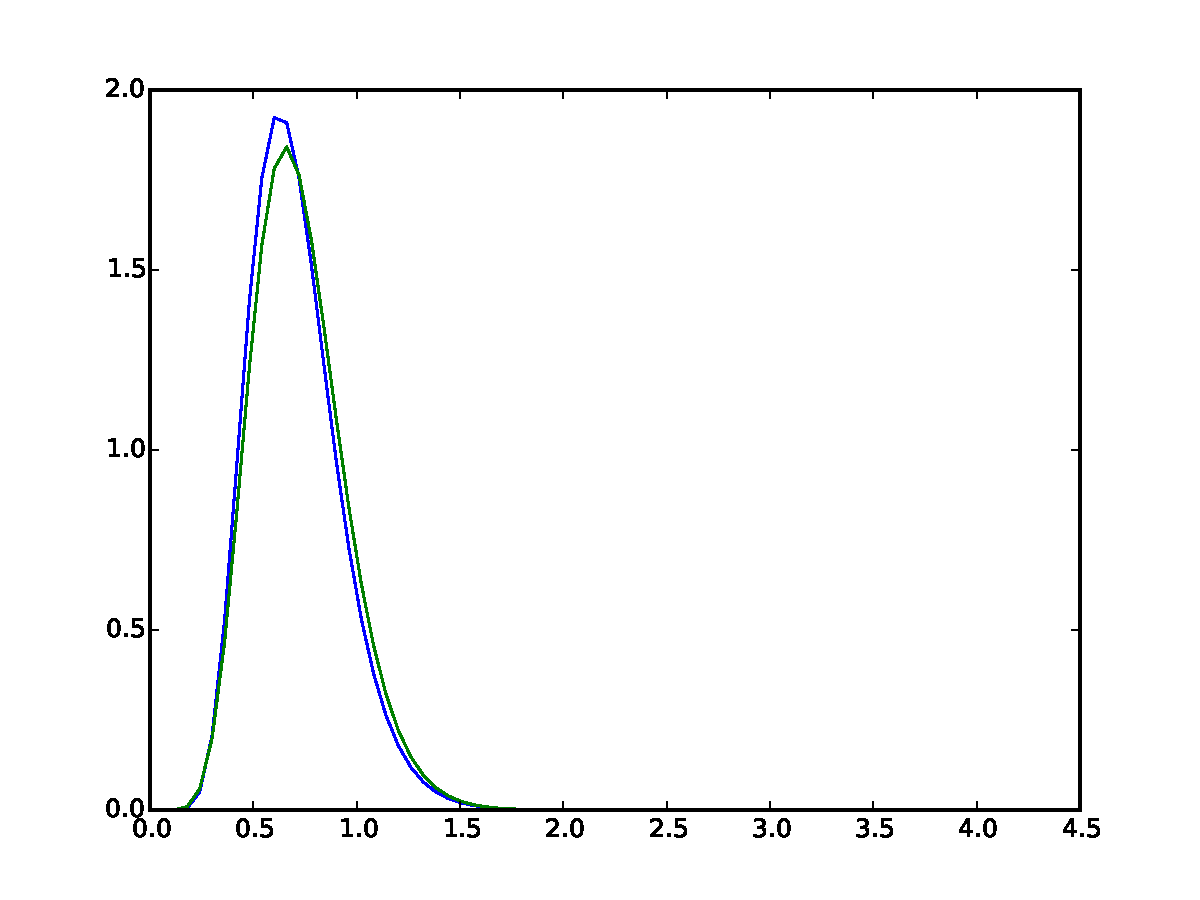
\includegraphics[width=0.97\linewidth]{bootstrap-filter/global_simple_3_3.pdf}
	\end{minipage}
	\begin{minipage}{.45\textwidth}
		\centering
		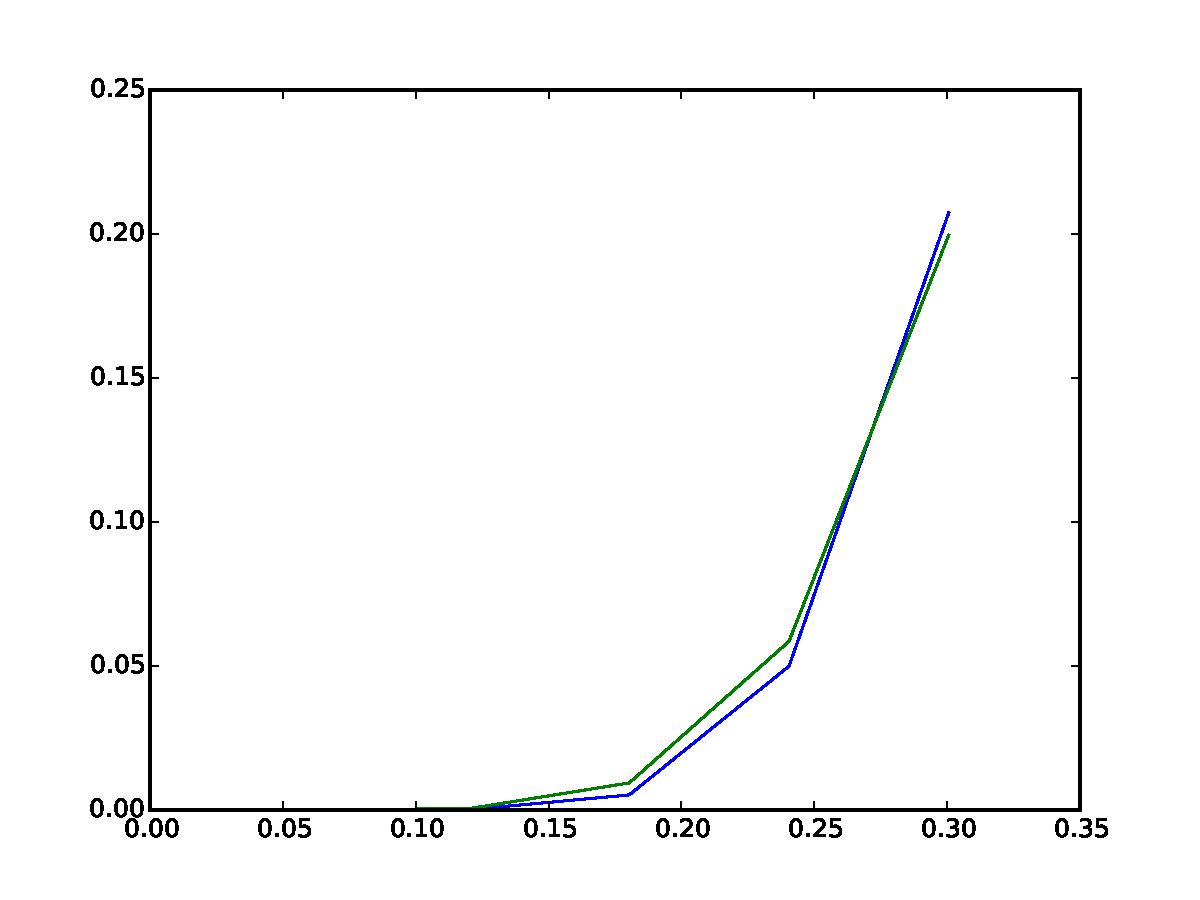
\includegraphics[width=0.97\linewidth]{bootstrap-filter/beginning_simple_3_3.pdf}
	\end{minipage}
	\begin{minipage}{.45\textwidth}
		\centering
		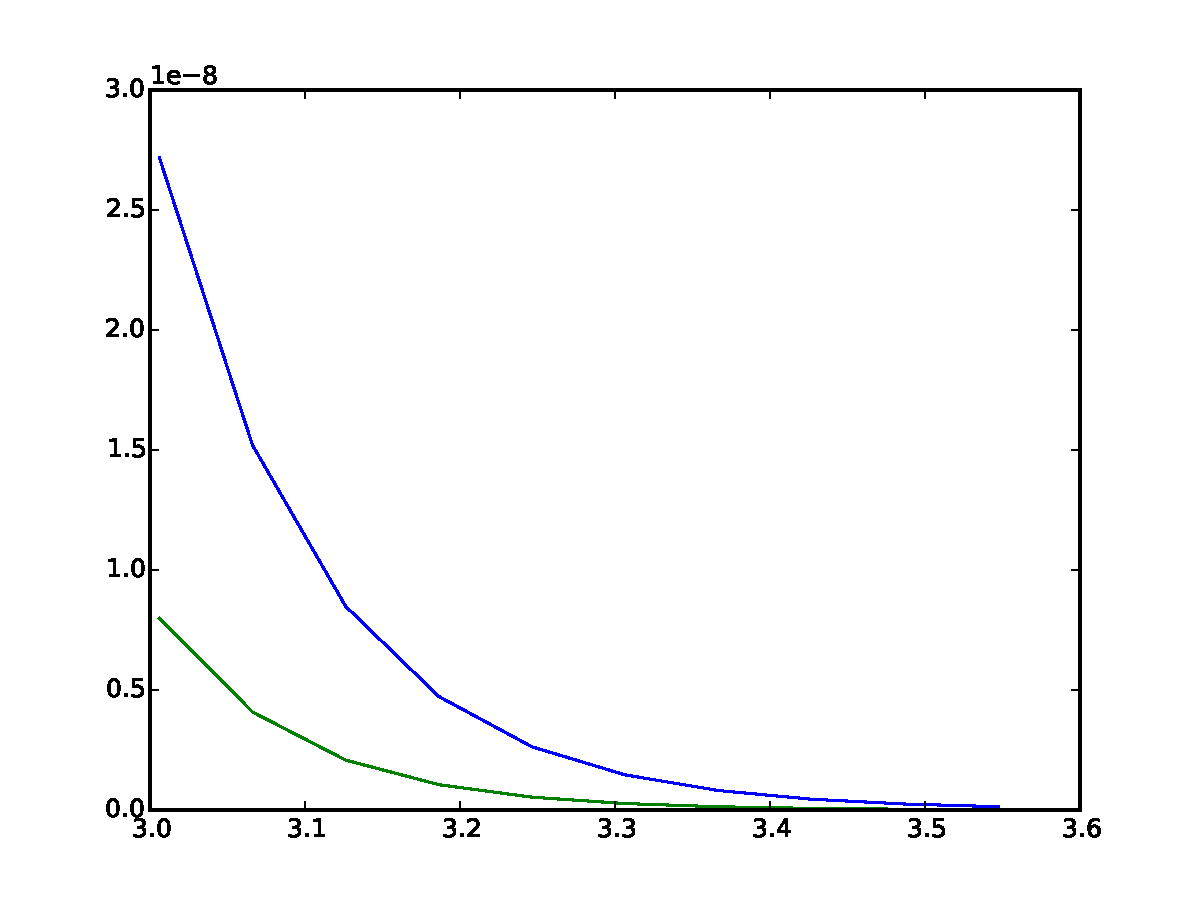
\includegraphics[width=0.97\linewidth]{bootstrap-filter/tail_simple_3_3.pdf}
	\end{minipage}
	\begin{minipage}{.45\textwidth}
		\centering
		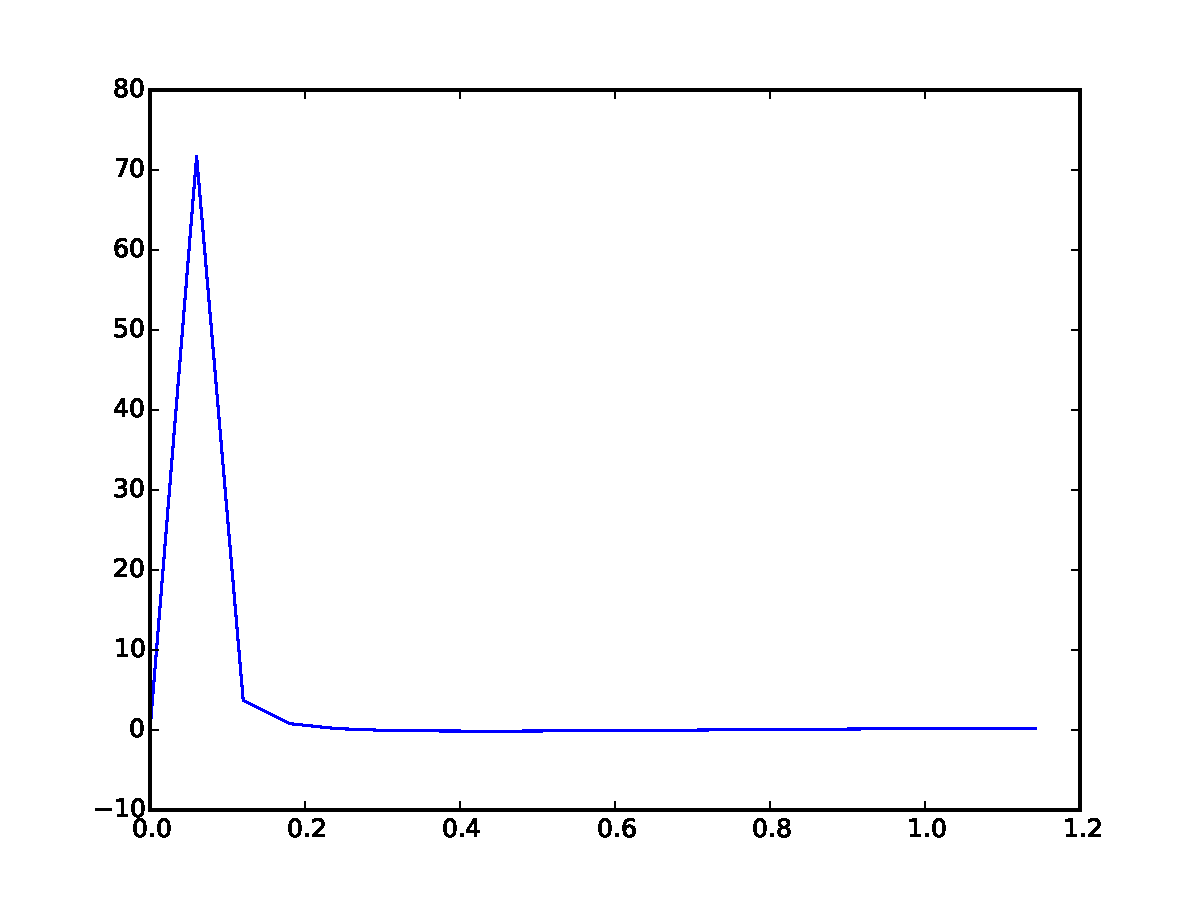
\includegraphics[width=0.97\linewidth]{bootstrap-filter/relative_beginning_simple_3_3.pdf}
	\end{minipage}
	\begin{minipage}{.45\textwidth}
		\centering
		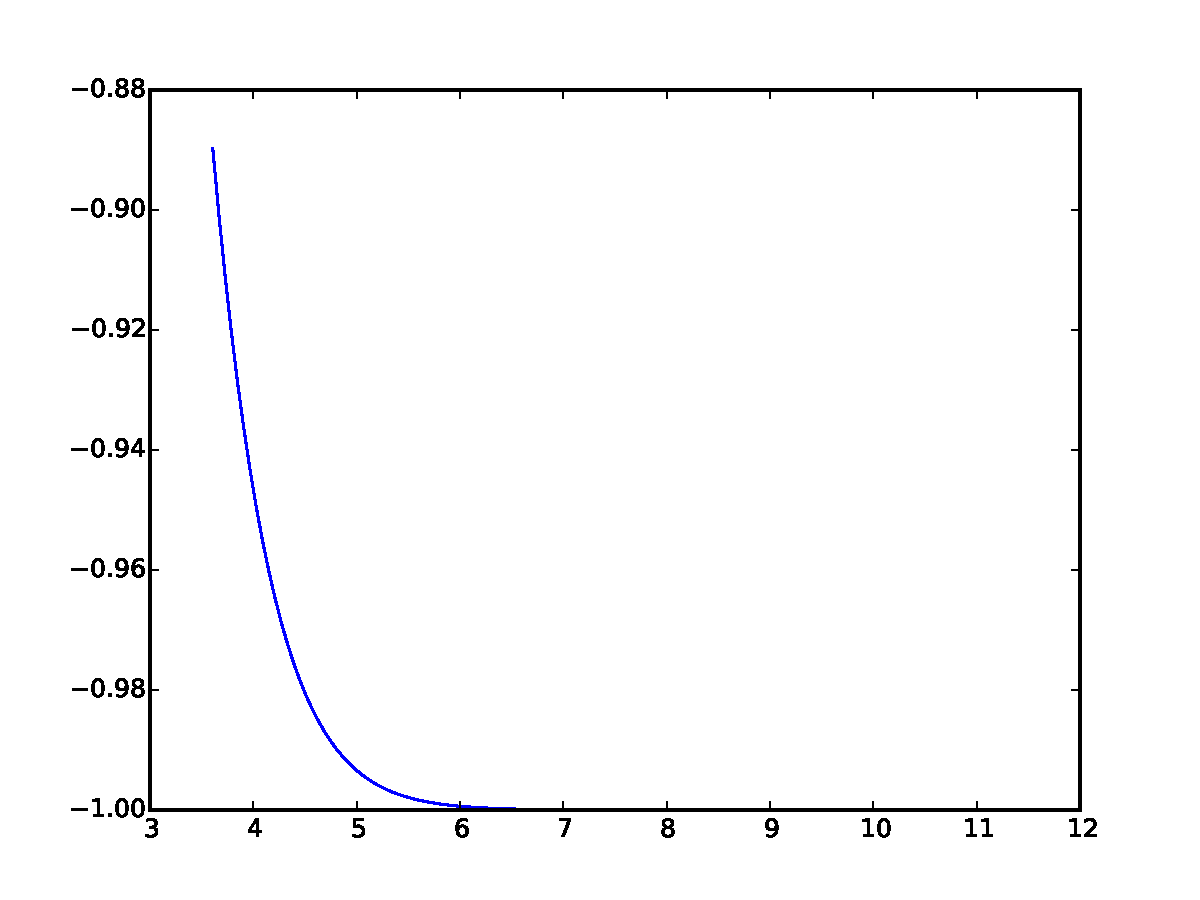
\includegraphics[width=0.97\linewidth]{bootstrap-filter/relative_tail_simple_3_3.pdf}
	\end{minipage}
	\begin{minipage}{.45\textwidth}
		\centering
		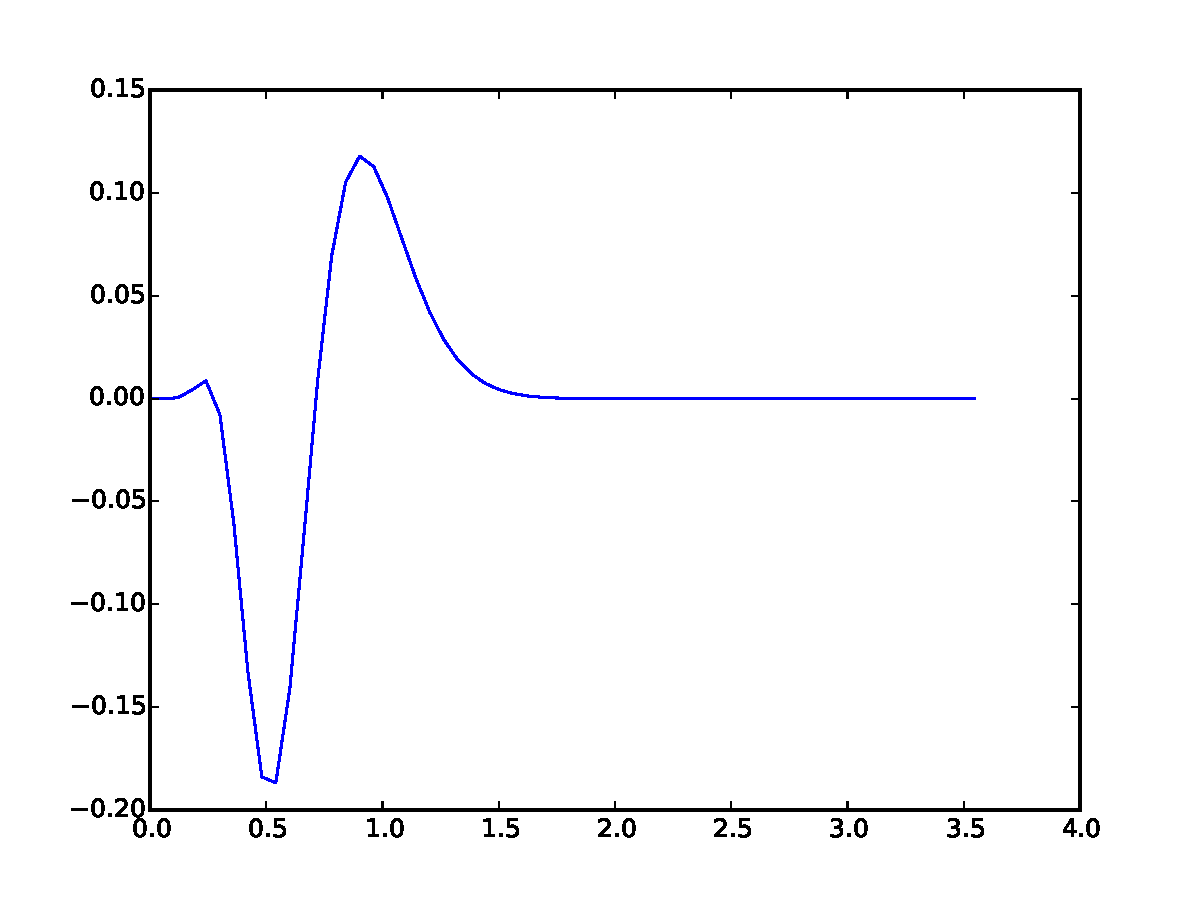
\includegraphics[width=0.97\linewidth]{bootstrap-filter/absolute_simple_3_3.pdf}
	\end{minipage}
	\caption{\textbf{(first row left)} Comparison between \textbf{(blue)} the optimal proposal density and \textbf{(green)} the gamma approximation density, \textbf{(first row right)} comparison between  the left tail of \textbf{(blue)} the optimal proposal density and of \textbf{(green)} the gamma approximation density, \textbf{(second row left)} comparison between the right tail of \textbf{(blue)} the optimal proposal density and of \textbf{(green)} the gamma approximation density, \textbf{(second row right)} relative error between values near 0 of the gamma approximation density and of the optimal proposal density, \textbf{(third row left)} relative error between the right tails of the gamma approximation density and of the optimal proposal density, \textbf{(third row right)} absolute error between the gamma approximation density and the optimal proposal density.}
	\label{fig:simple}
\end{figure}

\begin{figure}[htb]
	\centering
	\begin{minipage}{.45\textwidth}
		\centering
		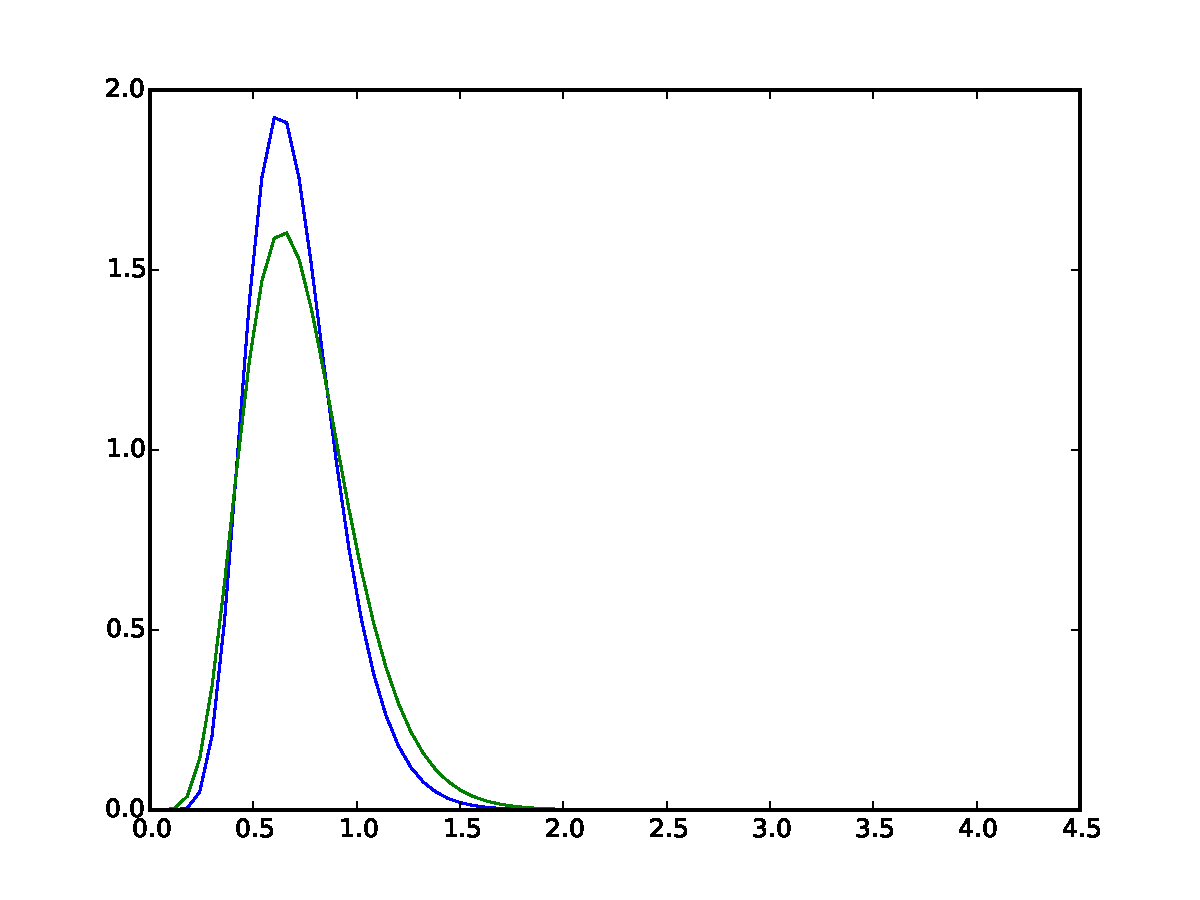
\includegraphics[width=0.97\linewidth]{bootstrap-filter/global_complex_3_3.pdf}
	\end{minipage}
	\begin{minipage}{.45\textwidth}
		\centering
		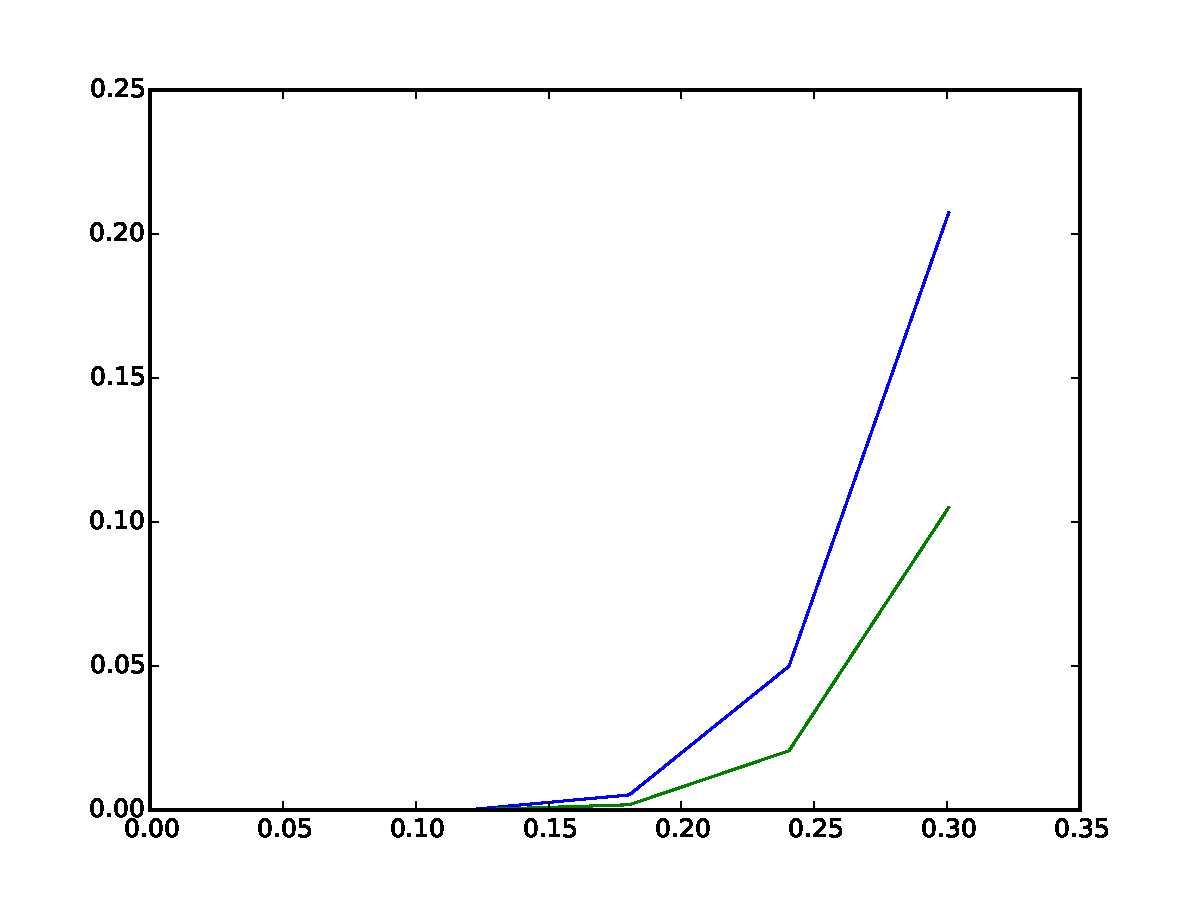
\includegraphics[width=0.97\linewidth]{bootstrap-filter/beginning_complex_3_3.pdf}
	\end{minipage}
	\begin{minipage}{.45\textwidth}
		\centering
		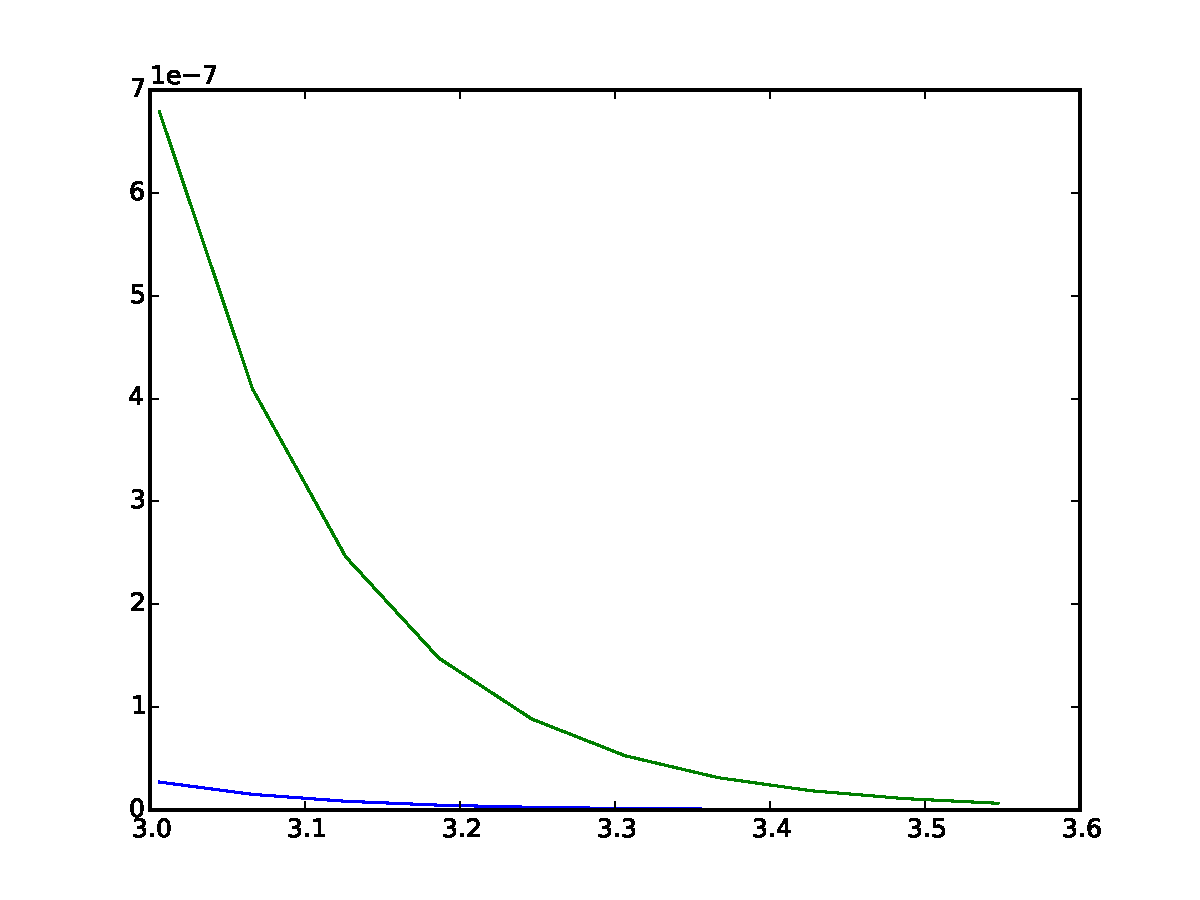
\includegraphics[width=0.97\linewidth]{bootstrap-filter/tail_complex_3_3.pdf}
	\end{minipage}
	\begin{minipage}{.45\textwidth}
		\centering
		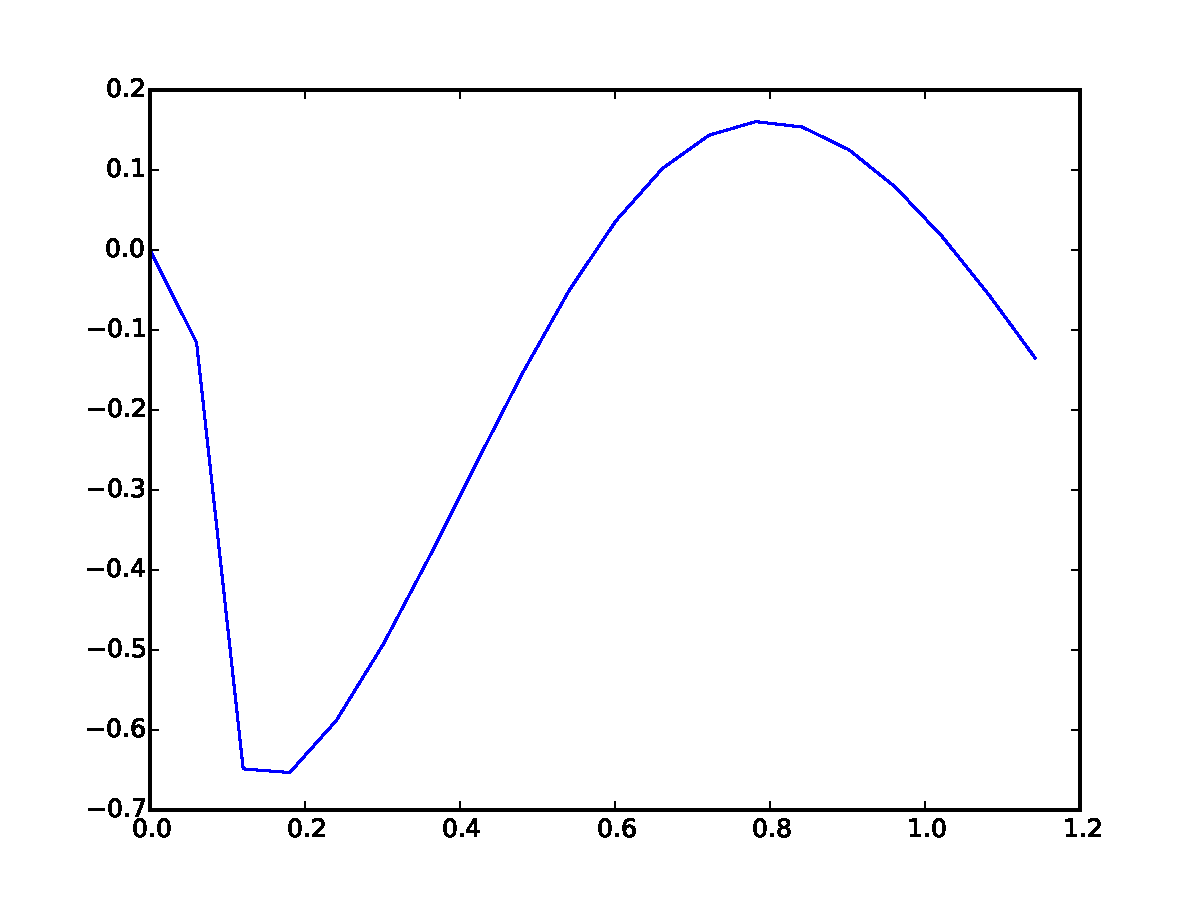
\includegraphics[width=0.97\linewidth]{bootstrap-filter/relative_beginning_complex_3_3.pdf}
	\end{minipage}
	\begin{minipage}{.45\textwidth}
		\centering
		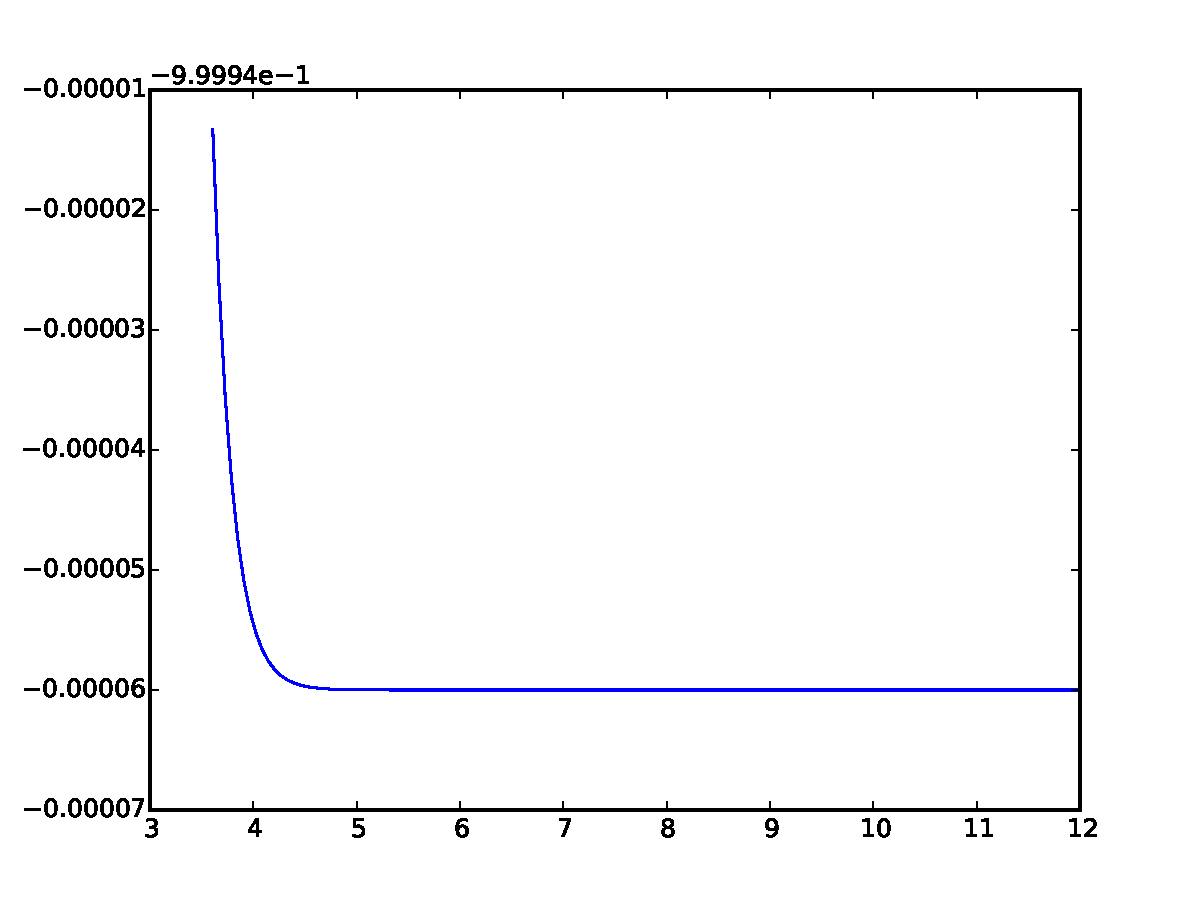
\includegraphics[width=0.97\linewidth]{bootstrap-filter/relative_tail_complex_3_3.pdf}
	\end{minipage}
	\begin{minipage}{.45\textwidth}
		\centering
		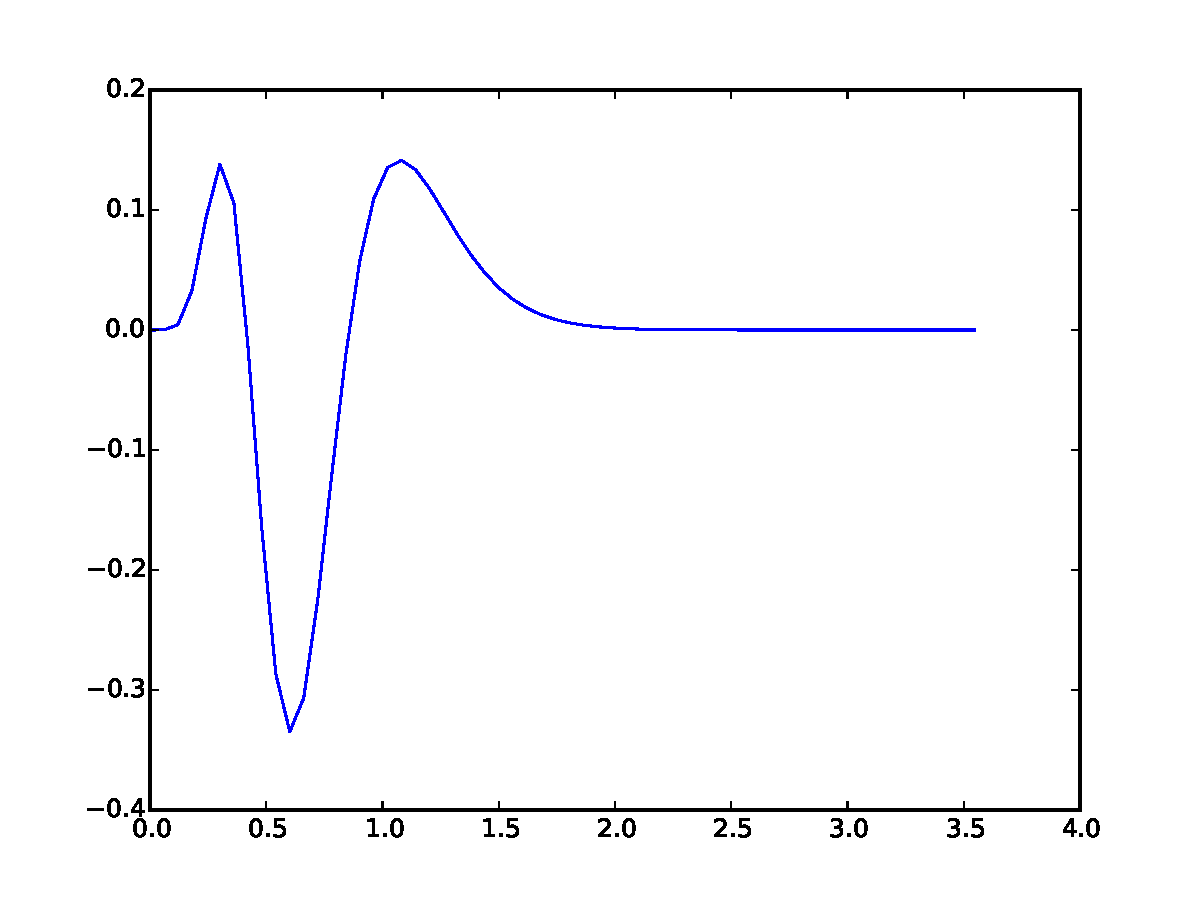
\includegraphics[width=0.97\linewidth]{bootstrap-filter/absolute_complex_3_3.pdf}
	\end{minipage}
	\caption{\textbf{(first row left)} Comparison between \textbf{(blue)} the optimal proposal density and \textbf{(green)} the gamma approximation density, \textbf{(first row right)} comparison between  the left tail of \textbf{(blue)} the optimal proposal density and of \textbf{(green)} the gamma approximation density, \textbf{(second row left)} comparison between the right tail of \textbf{(blue)} the optimal proposal density and of \textbf{(green)} the gamma approximation density, \textbf{(second row right)} relative error between values near 0 of the gamma approximation density and of the optimal proposal density, \textbf{(third row left)} relative error between the right tails of the gamma approximation density and of the optimal proposal density, \textbf{(third row right)} absolute error between the gamma approximation density and the optimal proposal density.}
	\label{fig:complex}
\end{figure}

\begin{figure}[htb]
	\centering
	\begin{minipage}{.3\textwidth}
		\centering
		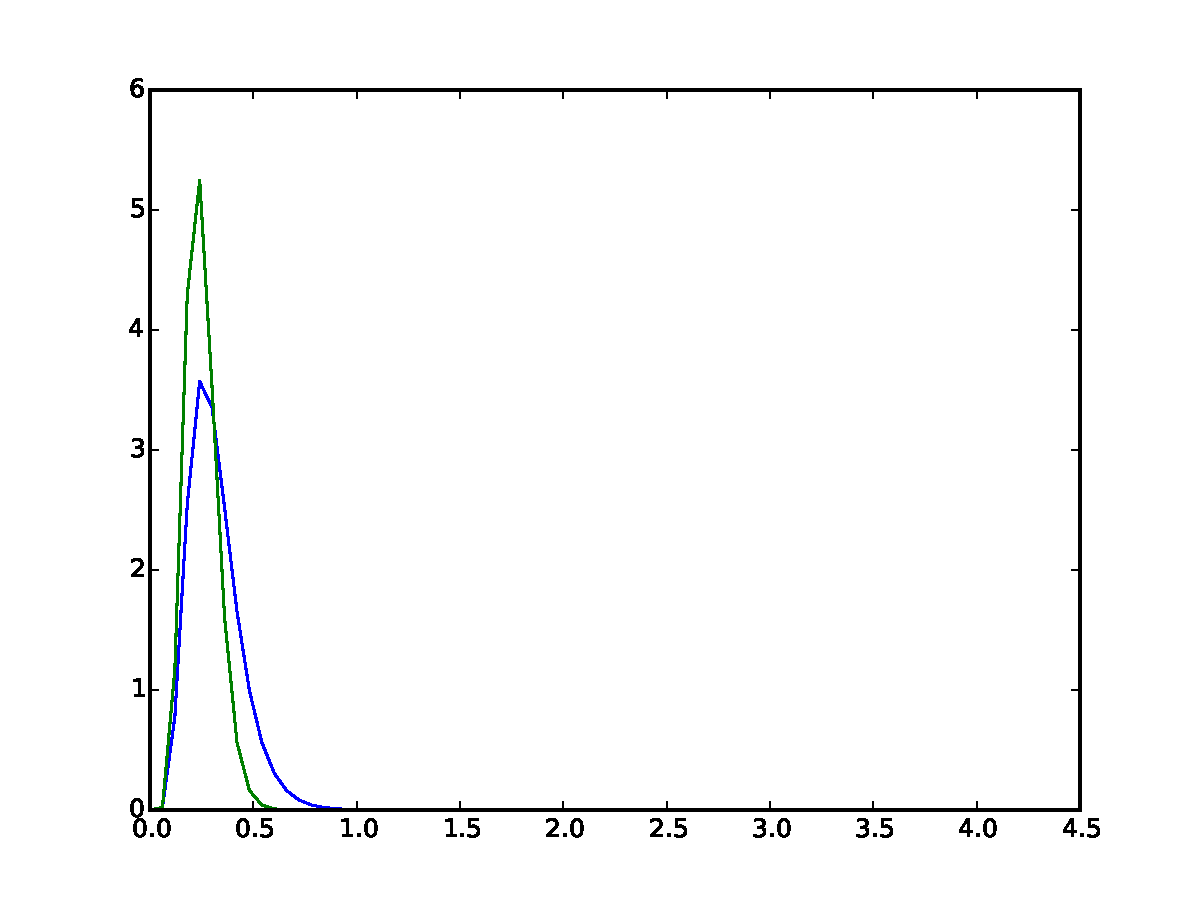
\includegraphics[width=0.97\linewidth]{bootstrap-filter/global_simple_1_3.pdf}
	\end{minipage}
	\begin{minipage}{.3\textwidth}
		\centering
		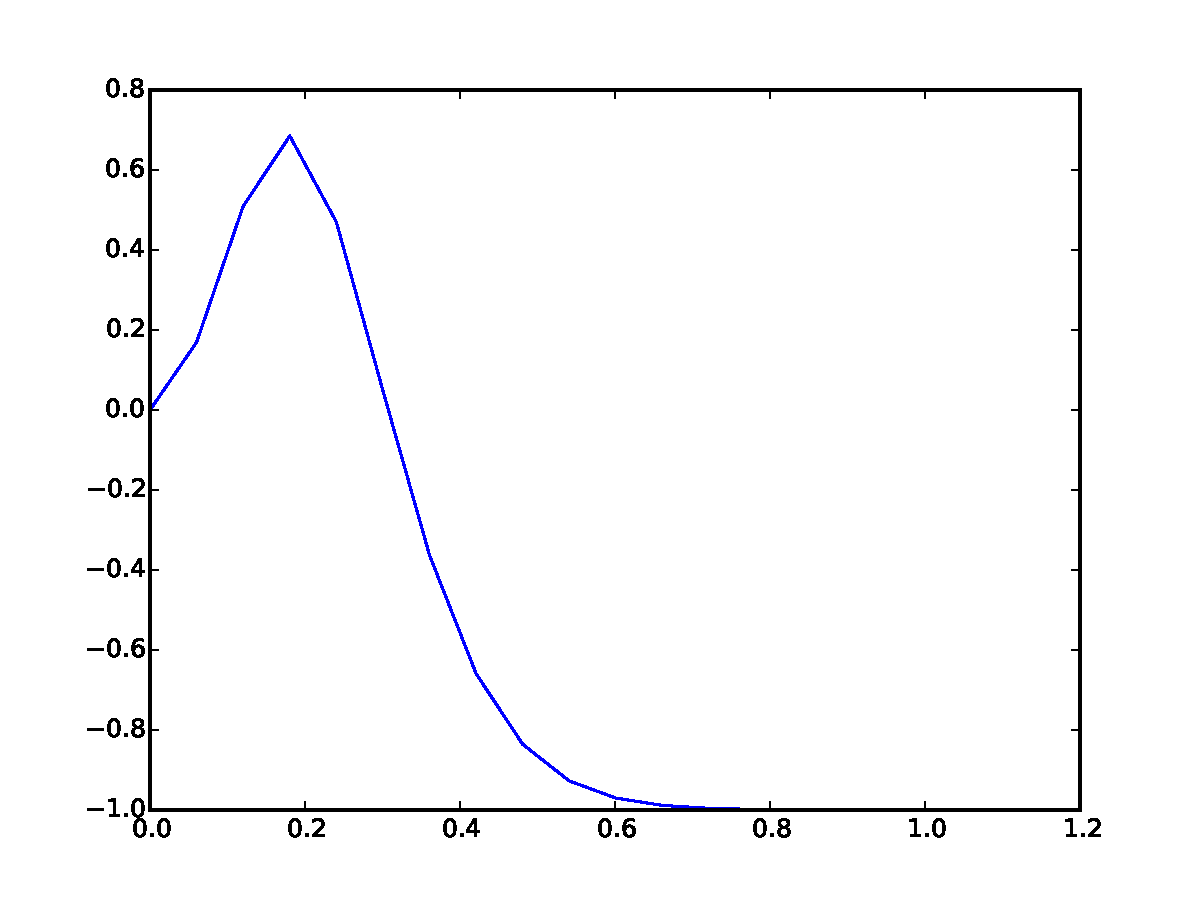
\includegraphics[width=0.97\linewidth]{bootstrap-filter/relative_beginning_simple_1_3.pdf}
	\end{minipage}
	\begin{minipage}{.3\textwidth}
		\centering
		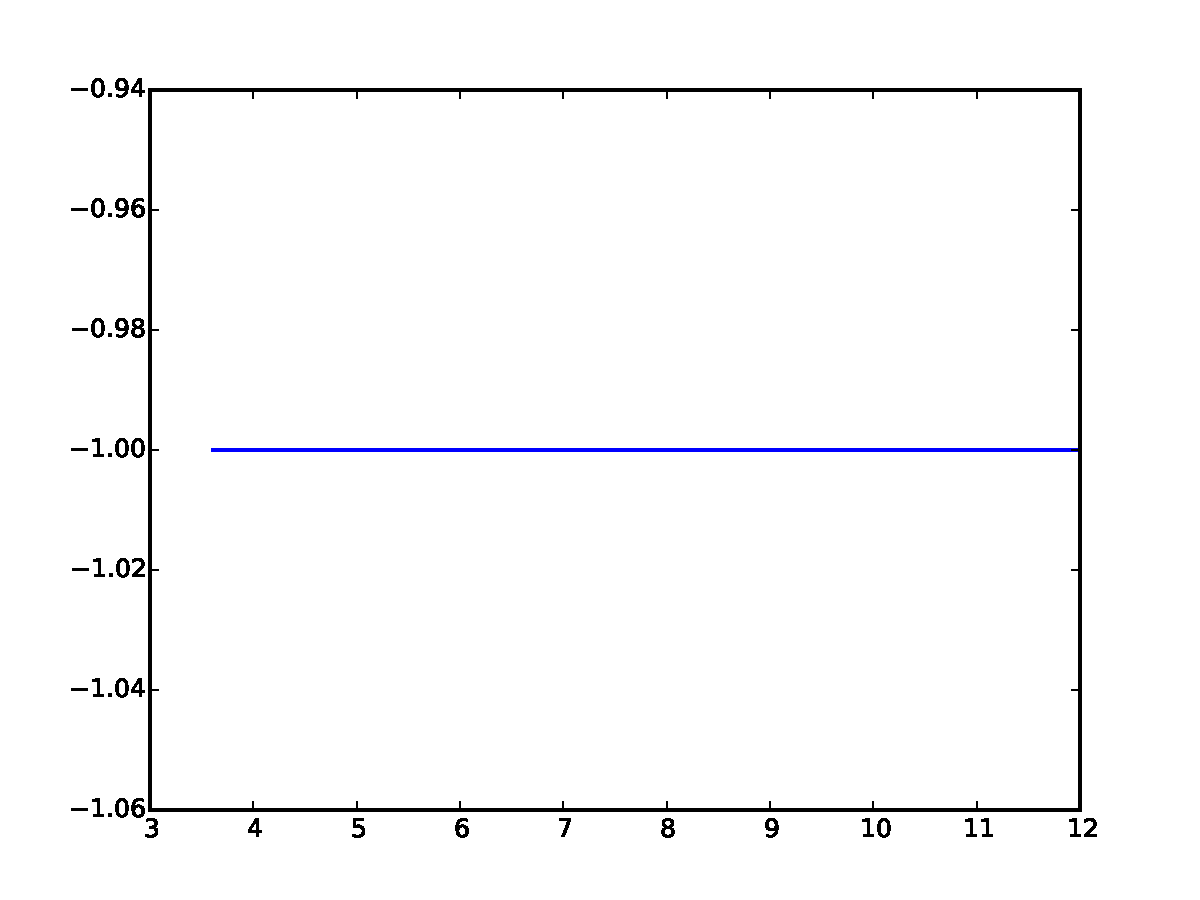
\includegraphics[width=0.97\linewidth]{bootstrap-filter/relative_tail_simple_1_3.pdf}
	\end{minipage}
	\begin{minipage}{.3\textwidth}
		\centering
		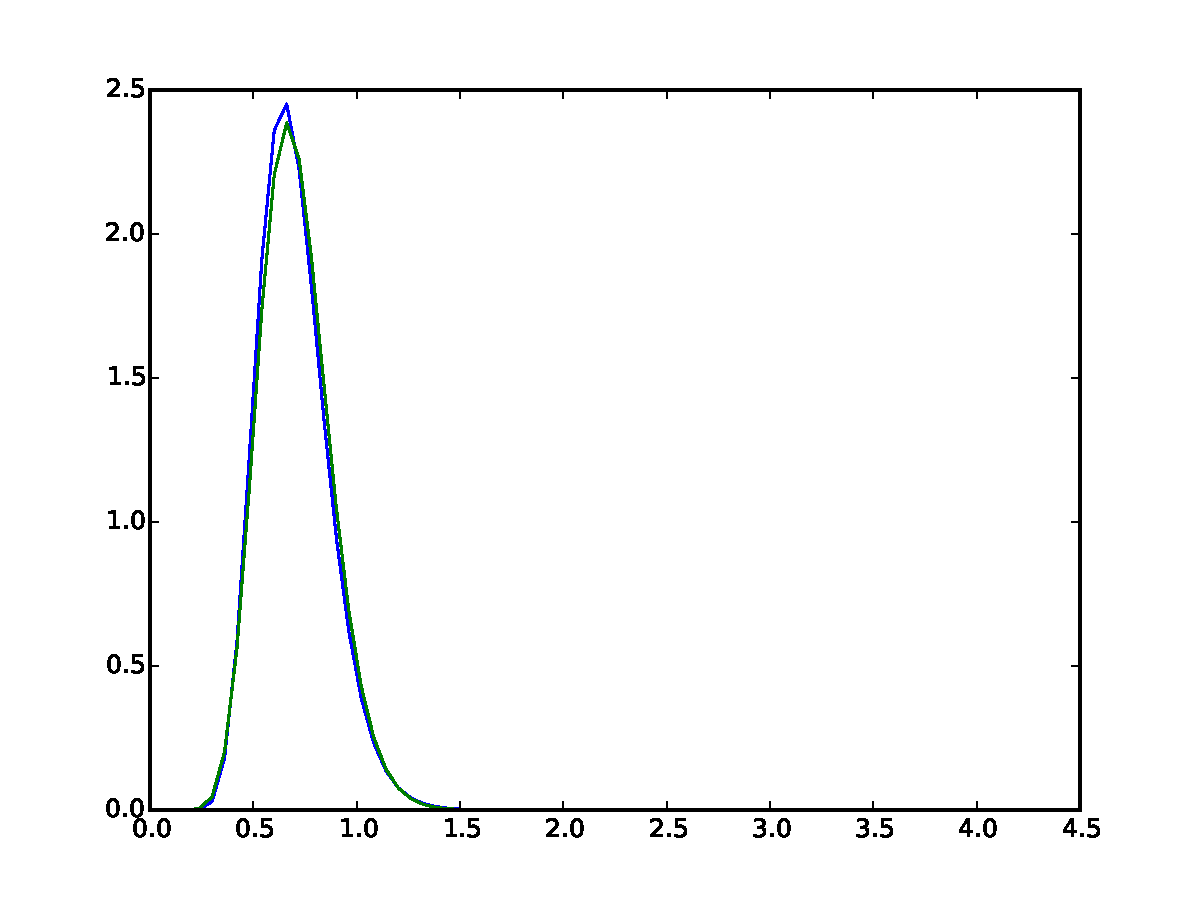
\includegraphics[width=0.97\linewidth]{bootstrap-filter/global_simple_3_1.pdf}
	\end{minipage}
	\begin{minipage}{.3\textwidth}
		\centering
		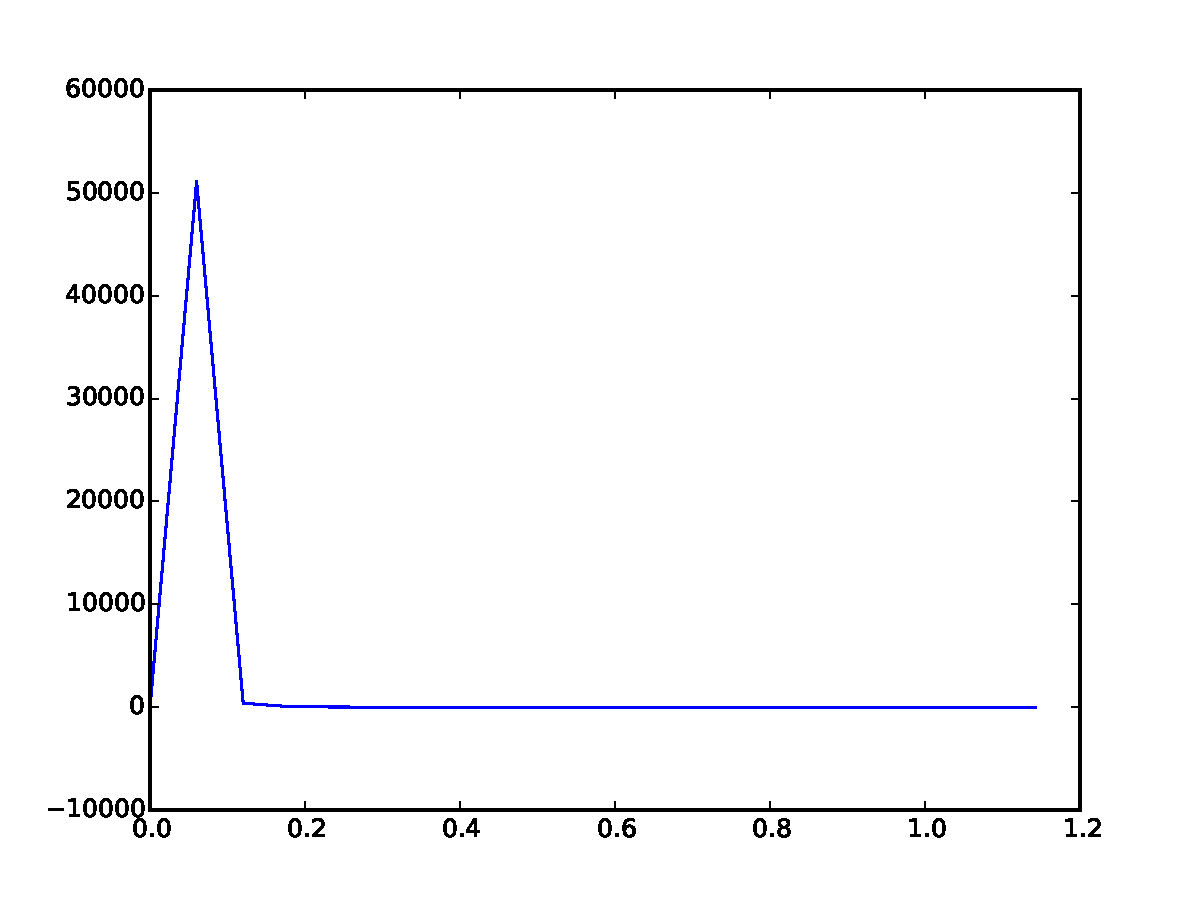
\includegraphics[width=0.97\linewidth]{bootstrap-filter/relative_beginning_simple_4_3.pdf}
	\end{minipage}
	\begin{minipage}{.3\textwidth}
		\centering
		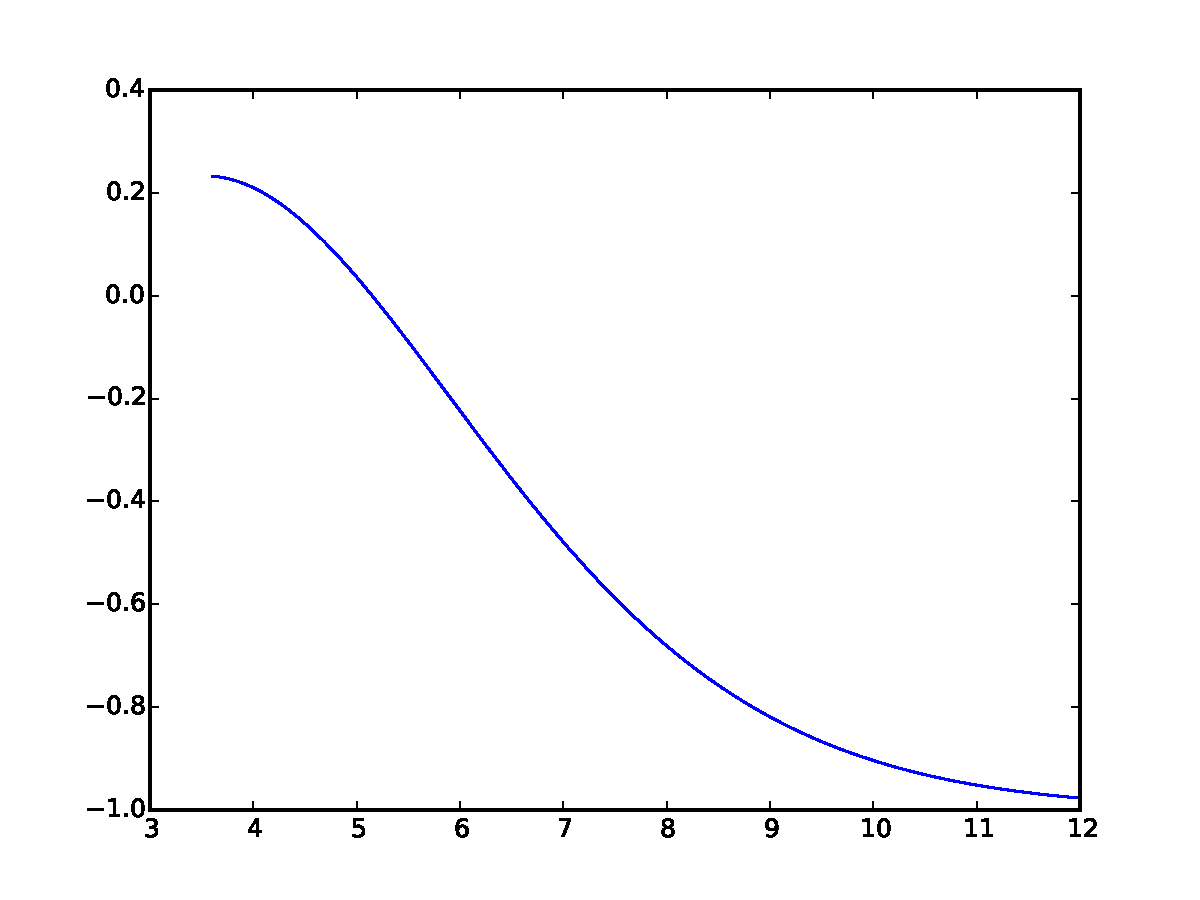
\includegraphics[width=0.97\linewidth]{bootstrap-filter/relative_tail_simple_4_3.pdf}
	\end{minipage}
	\begin{minipage}{.3\textwidth}
		\centering
		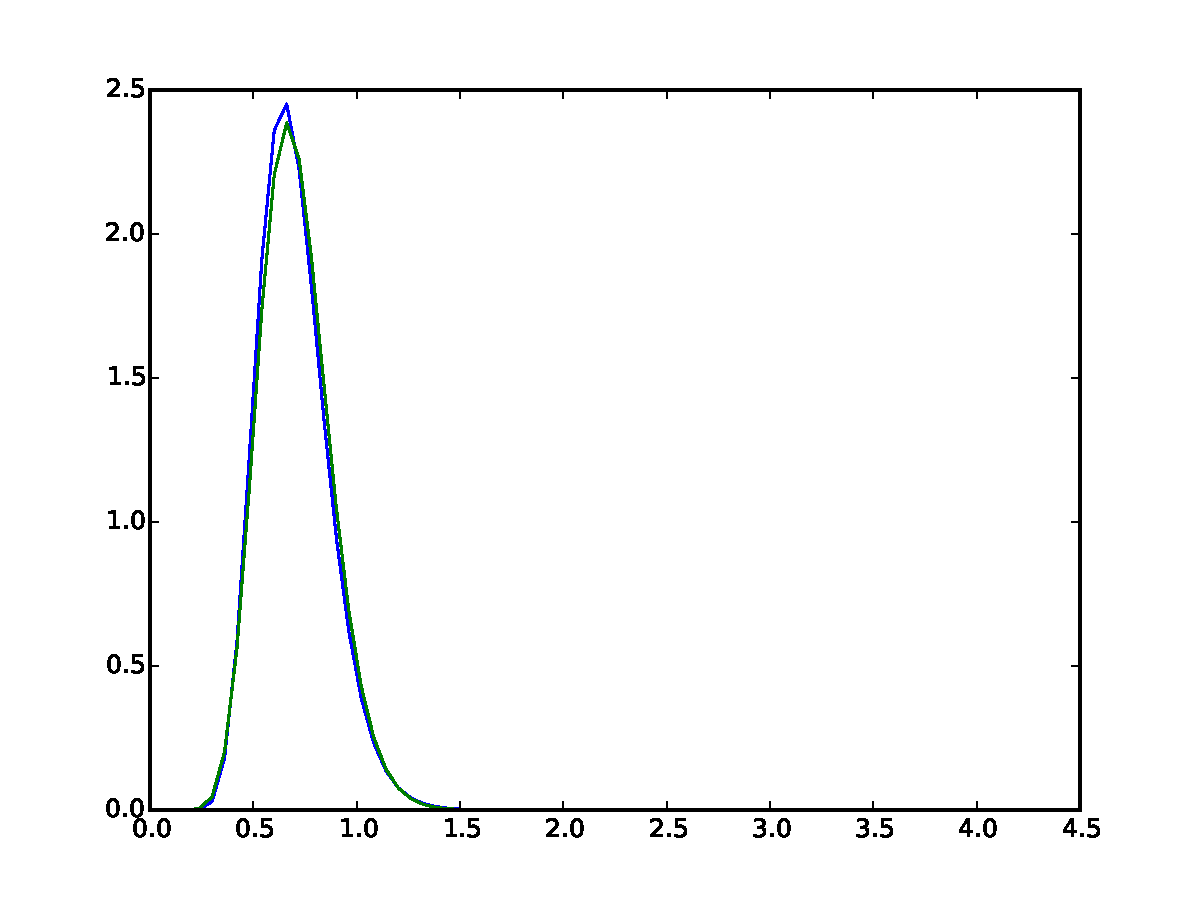
\includegraphics[width=0.97\linewidth]{bootstrap-filter/global_simple_3_1.pdf}
	\end{minipage}
	\begin{minipage}{.3\textwidth}
		\centering
		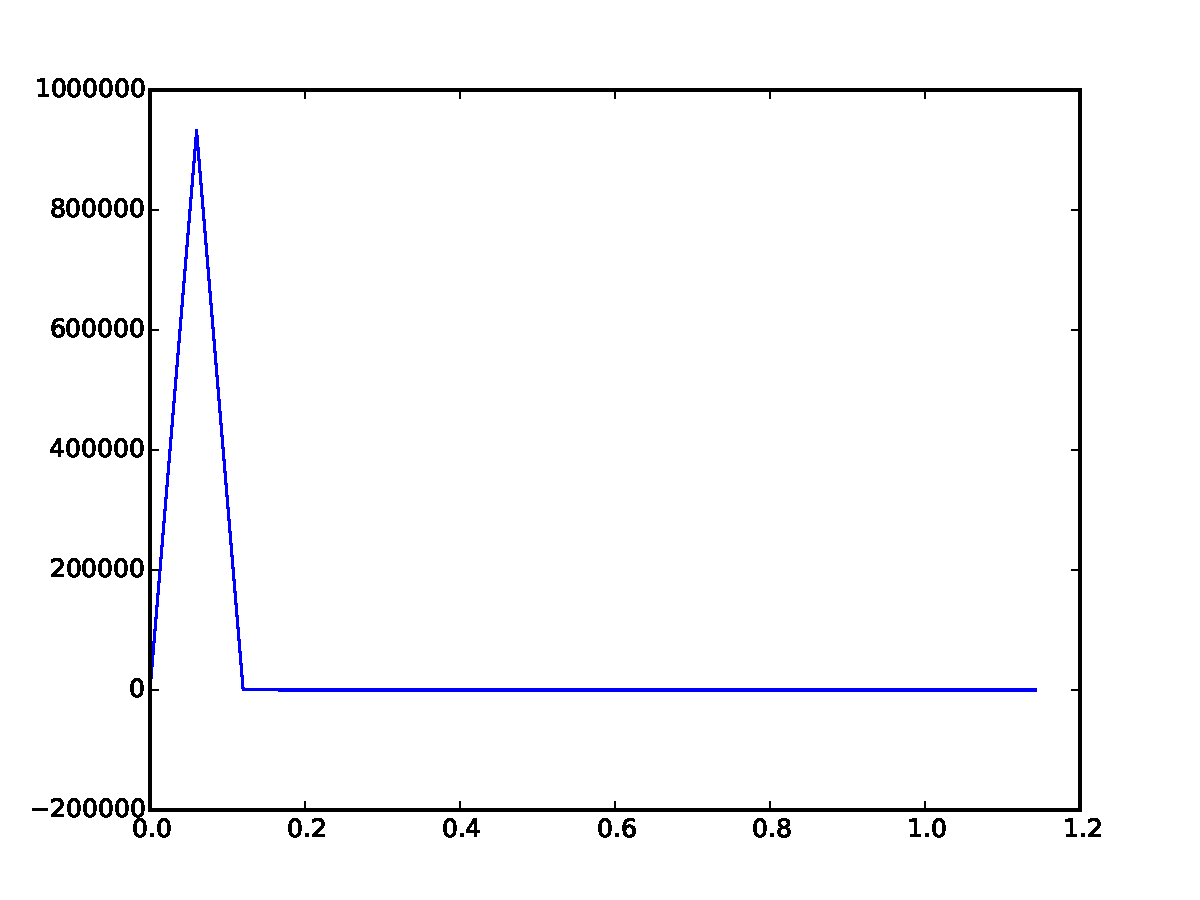
\includegraphics[width=0.97\linewidth]{bootstrap-filter/relative_beginning_simple_3_1.pdf}
	\end{minipage}
	\begin{minipage}{.3\textwidth}
		\centering
		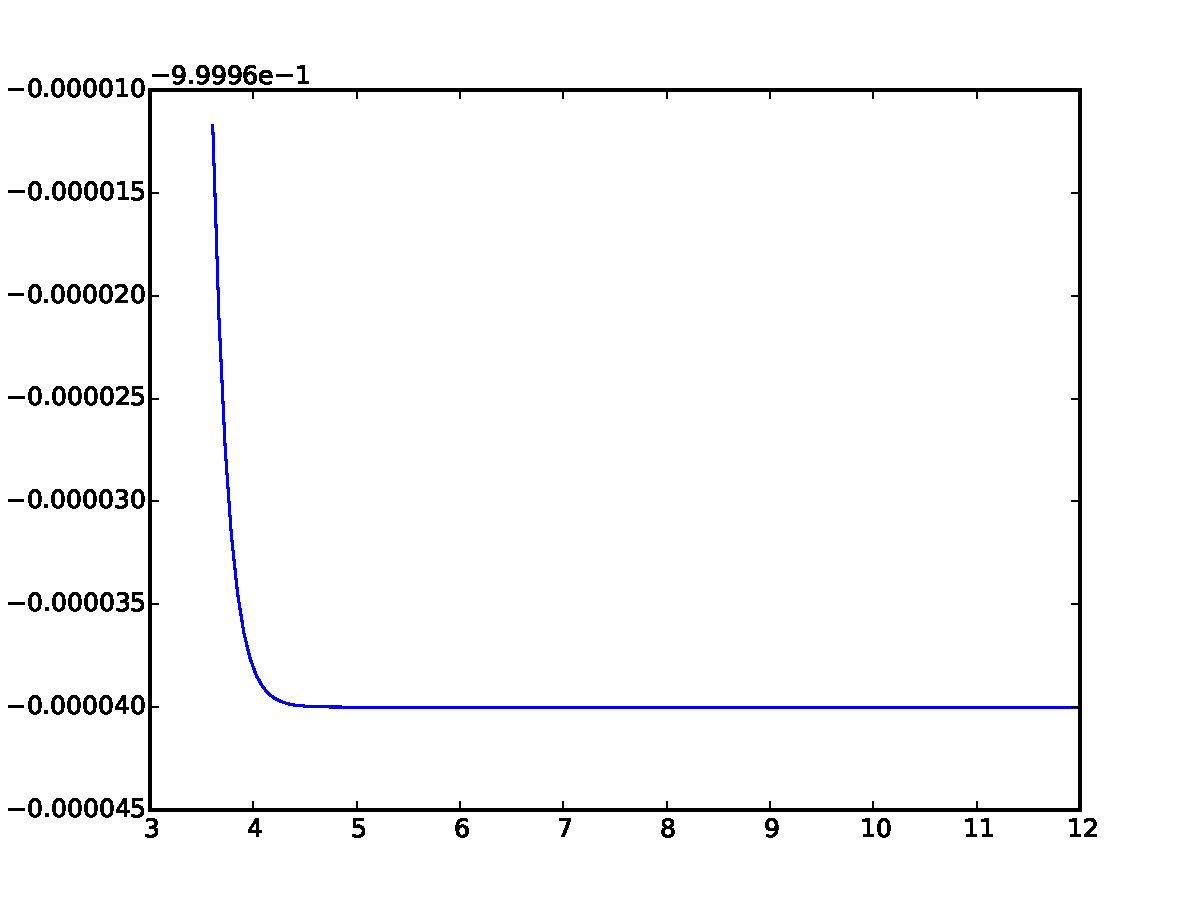
\includegraphics[width=0.97\linewidth]{bootstrap-filter/relative_tail_simple_3_1.pdf}
	\end{minipage}
	\begin{minipage}{.3\textwidth}
		\centering
		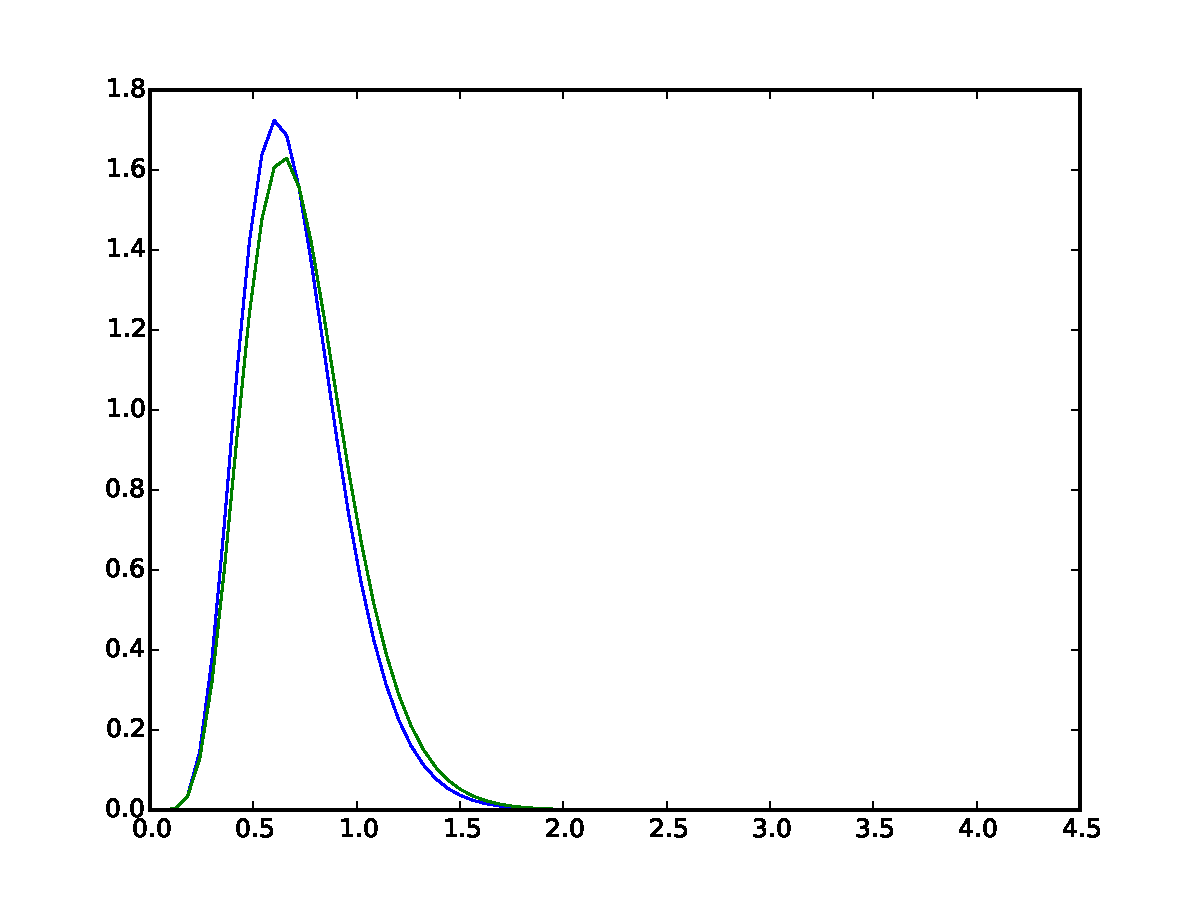
\includegraphics[width=0.97\linewidth]{bootstrap-filter/global_simple_3_9.pdf}
	\end{minipage}
	\begin{minipage}{.3\textwidth}
		\centering
		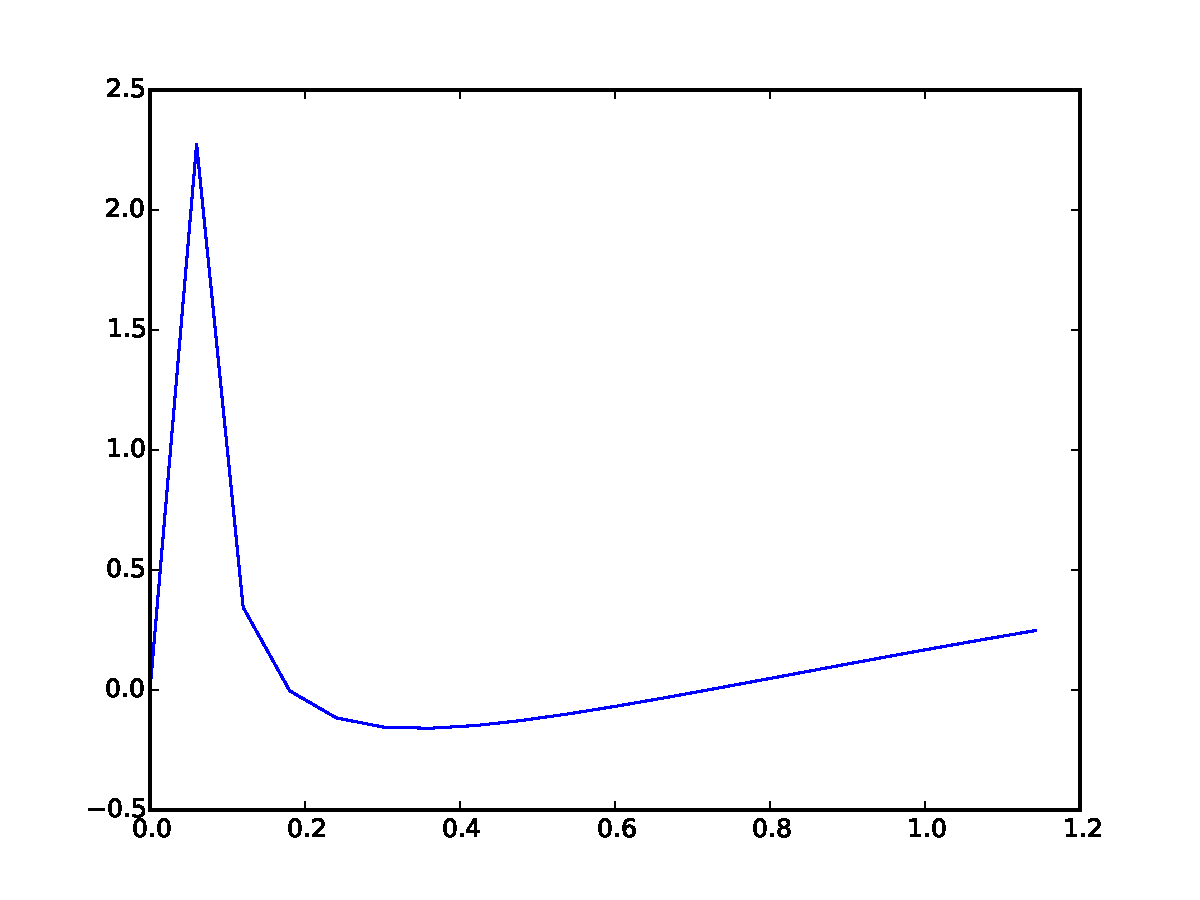
\includegraphics[width=0.97\linewidth]{bootstrap-filter/relative_beginning_simple_3_9.pdf}
	\end{minipage}
	\begin{minipage}{.3\textwidth}
		\centering
		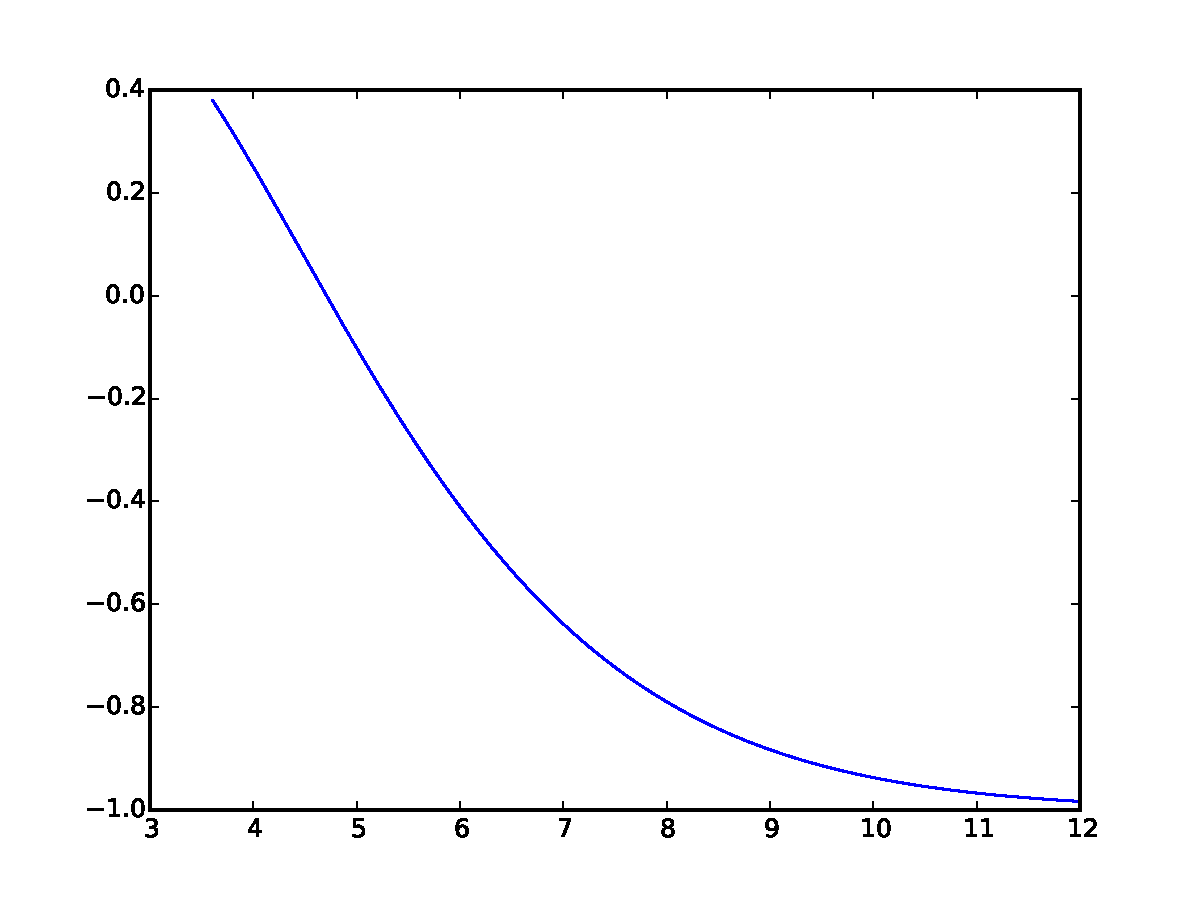
\includegraphics[width=0.97\linewidth]{bootstrap-filter/relative_tail_simple_3_9.pdf}
	\end{minipage}
	\caption{\textbf{(left)} Comparison between \textbf{(blue)} the optimal proposal density and \textbf{(green)} the gamma approximation density, \textbf{(middle)} relative error between values near 0 of the gamma approximation density and the optimal proposal density, \textbf{(right)} relative error between the right tails of the gamma approximation density and the optimal proposal density for \textbf{(first row)} $\ln(r)=1$ and $\sigma^2 = 0.3$, \textbf{(second row)} $\ln(r)=4$ and $\sigma^2 = 0.3$, \textbf{(third row)} $\ln(r)=3$ and $\sigma^2 = 0.1$, \textbf{(fourth row)} $\ln(r)=3$ and $\sigma^2 = 0.9$.}
	\label{fig:movingsimple}
\end{figure}

\begin{figure}[htb]
	\centering
	\begin{minipage}{.3\textwidth}
		\centering
		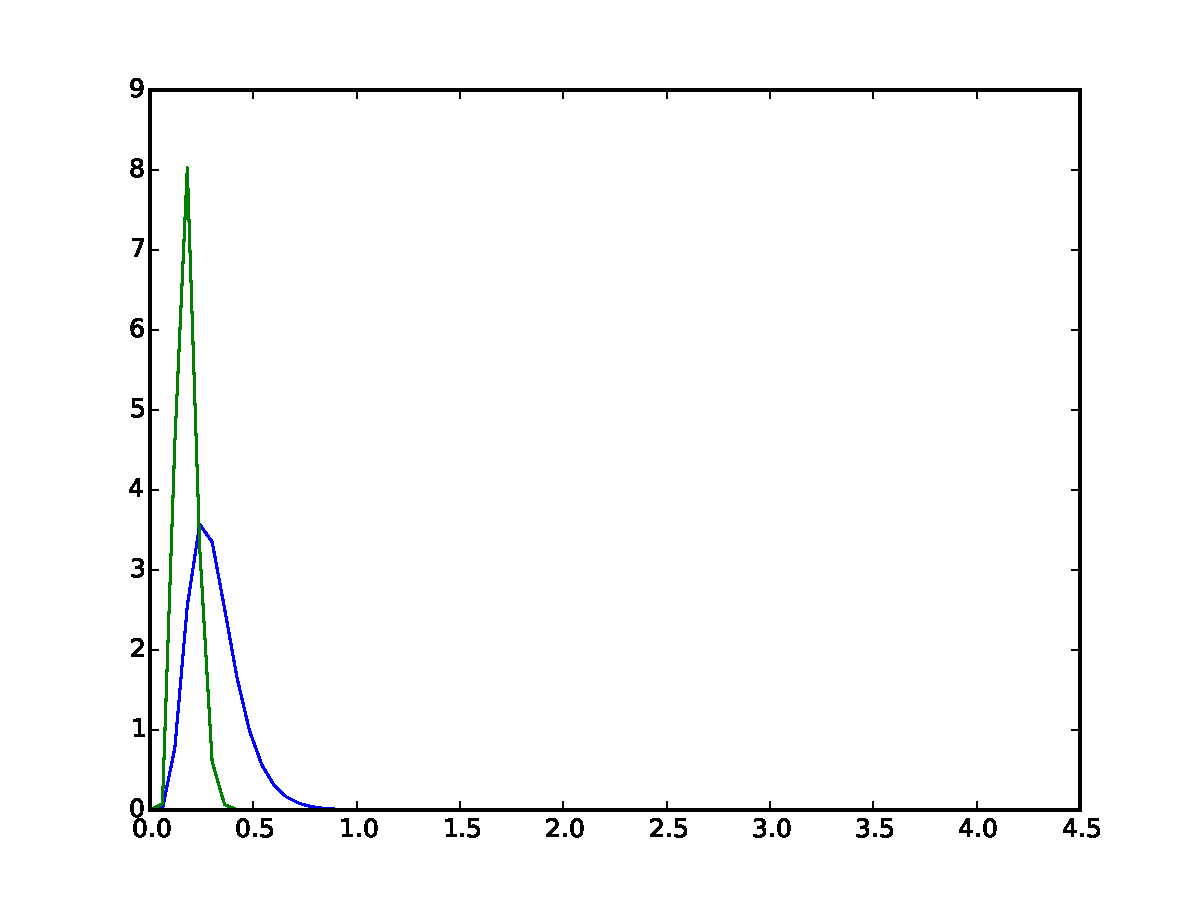
\includegraphics[width=0.97\linewidth]{bootstrap-filter/global_complex_1_3.pdf}
	\end{minipage}
	\begin{minipage}{.3\textwidth}
		\centering
		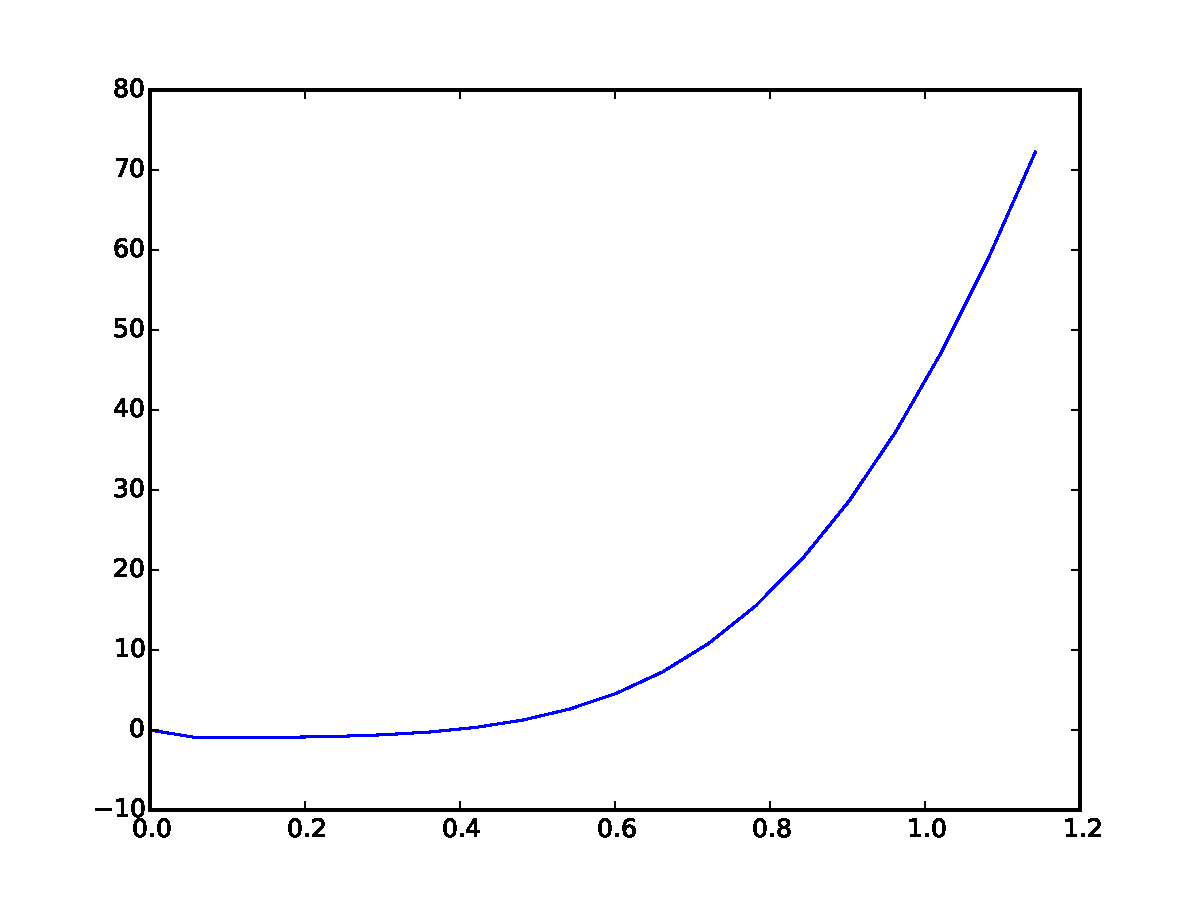
\includegraphics[width=0.97\linewidth]{bootstrap-filter/relative_beginning_complex_1_3.pdf}
	\end{minipage}
	\begin{minipage}{.3\textwidth}
		\centering
		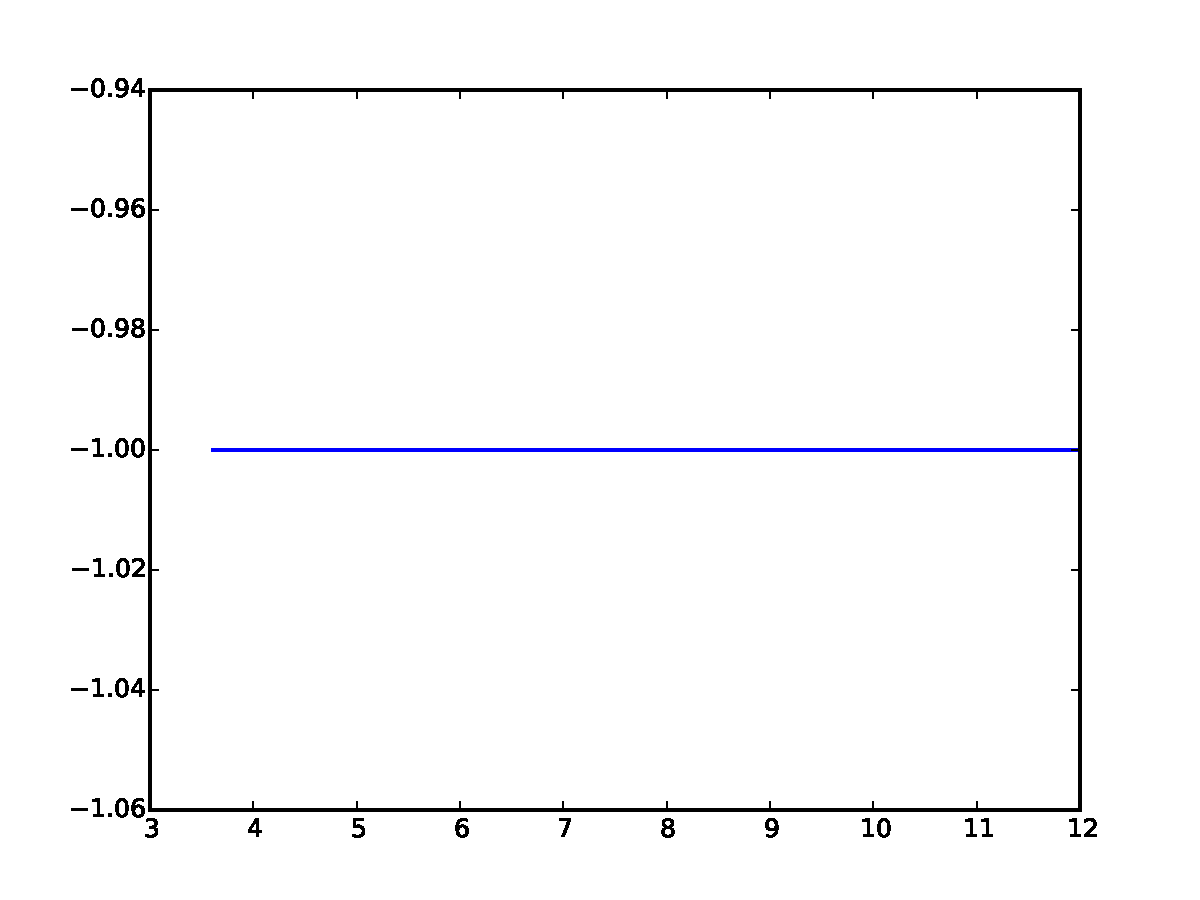
\includegraphics[width=0.97\linewidth]{bootstrap-filter/relative_tail_complex_1_3.pdf}
	\end{minipage}
	\begin{minipage}{.3\textwidth}
		\centering
		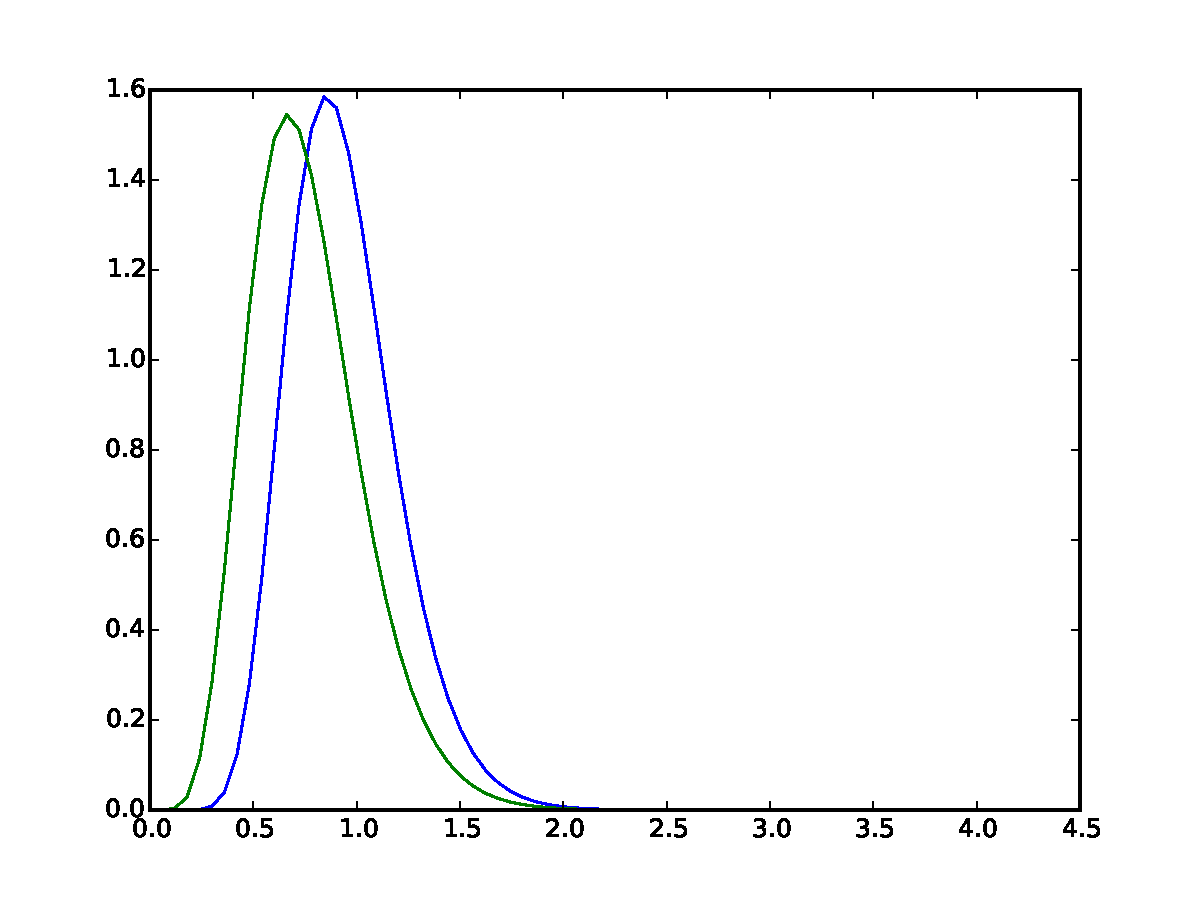
\includegraphics[width=0.97\linewidth]{bootstrap-filter/global_complex_4_3.pdf}
	\end{minipage}
	\begin{minipage}{.3\textwidth}
		\centering
		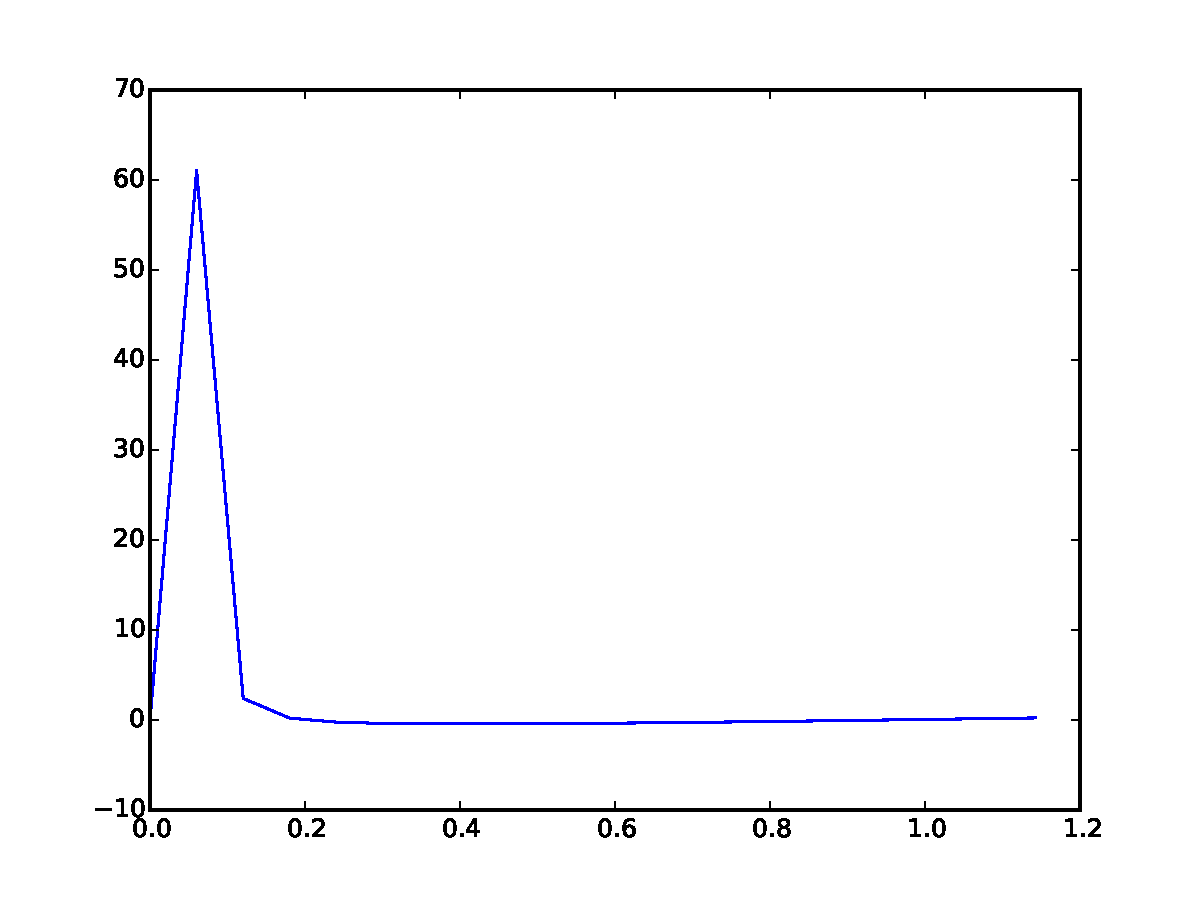
\includegraphics[width=0.97\linewidth]{bootstrap-filter/relative_beginning_complex_4_3.pdf}
	\end{minipage}
	\begin{minipage}{.3\textwidth}
		\centering
		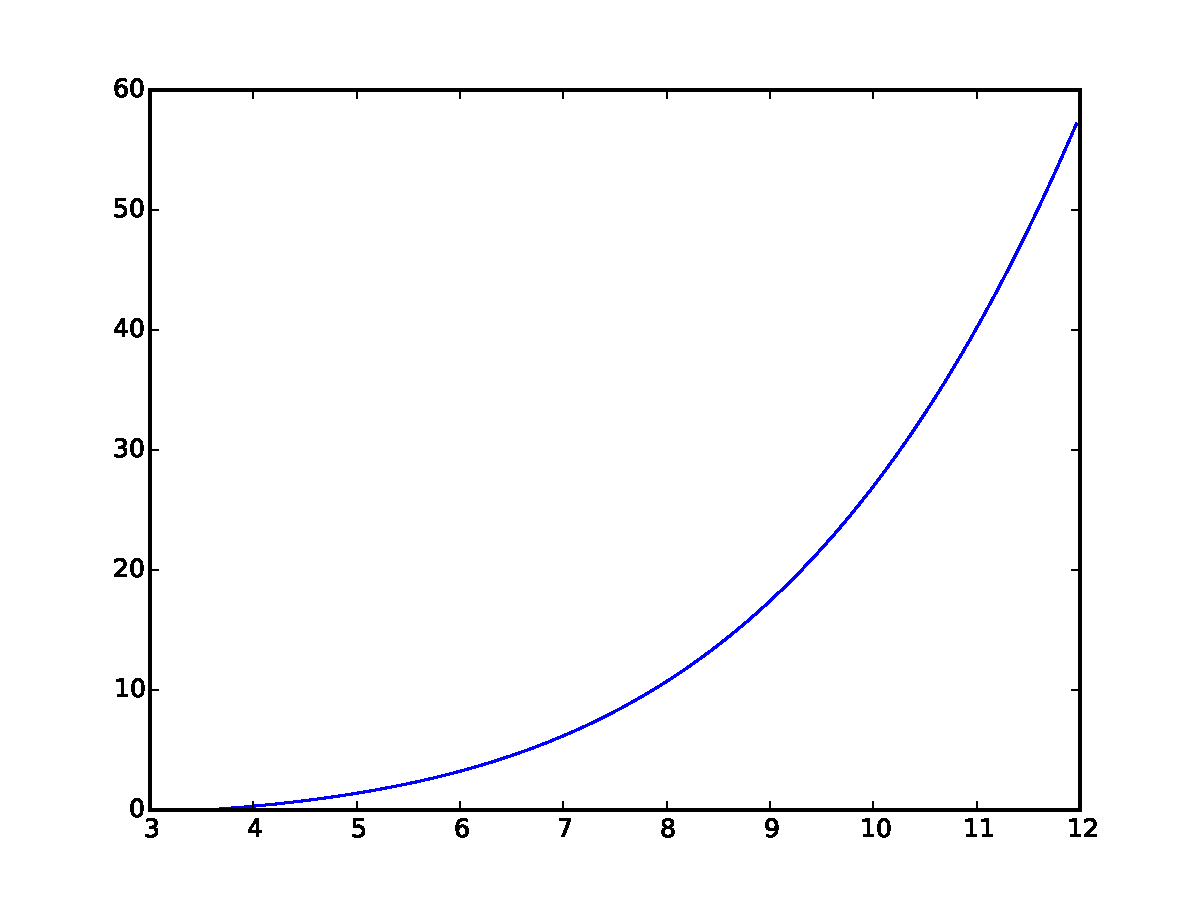
\includegraphics[width=0.97\linewidth]{bootstrap-filter/relative_tail_complex_4_3.pdf}
	\end{minipage}
	\begin{minipage}{.3\textwidth}
		\centering
		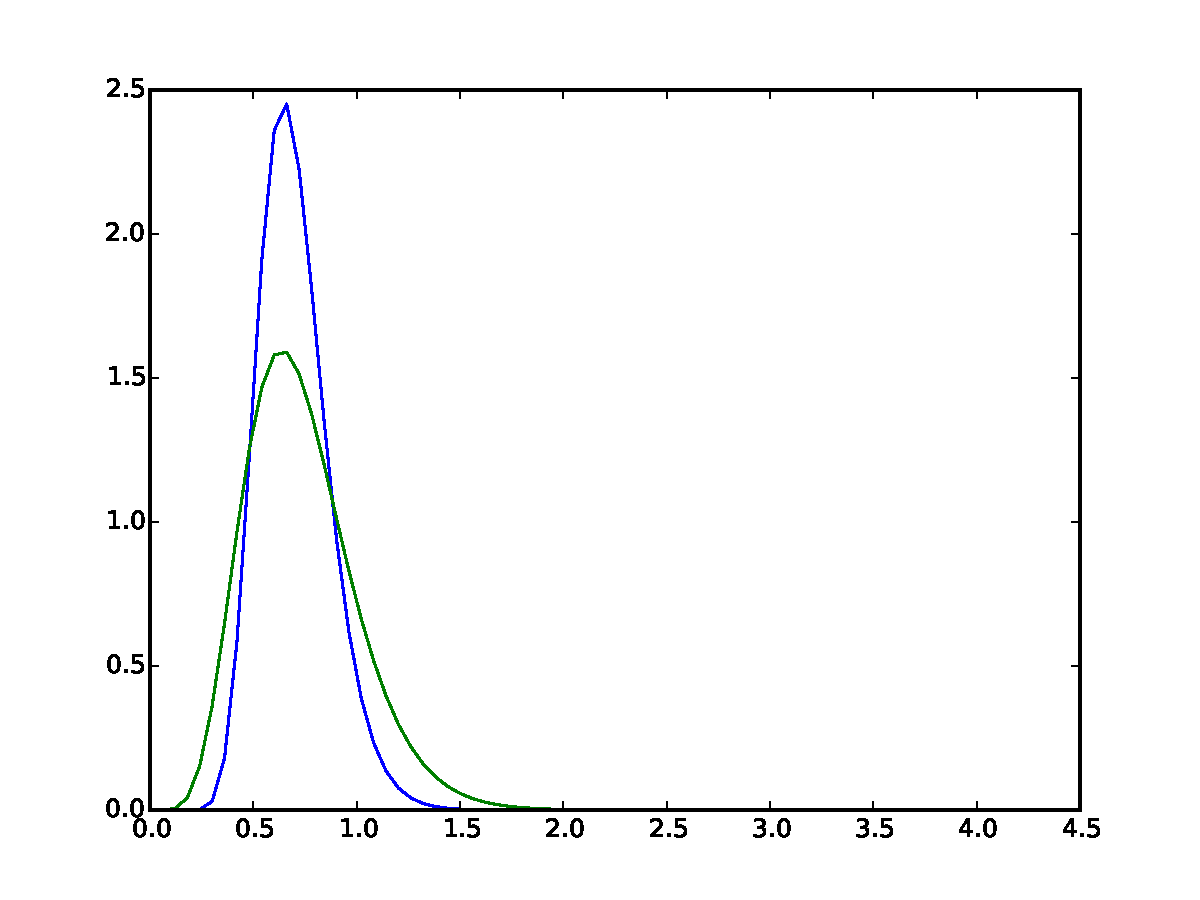
\includegraphics[width=0.97\linewidth]{bootstrap-filter/global_complex_3_1.pdf}
	\end{minipage}
	\begin{minipage}{.3\textwidth}
		\centering
		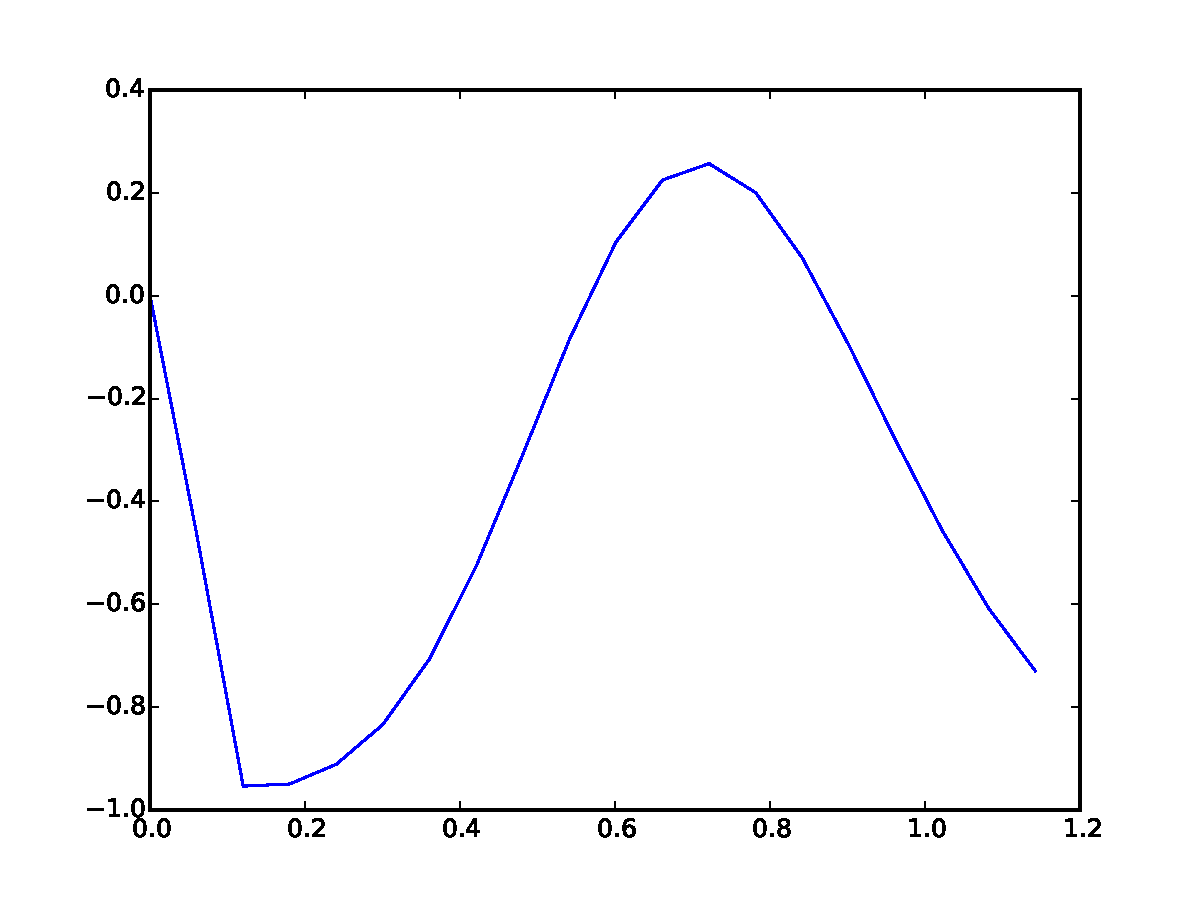
\includegraphics[width=0.97\linewidth]{bootstrap-filter/relative_beginning_complex_3_1.pdf}
	\end{minipage}
	\begin{minipage}{.3\textwidth}
		\centering
		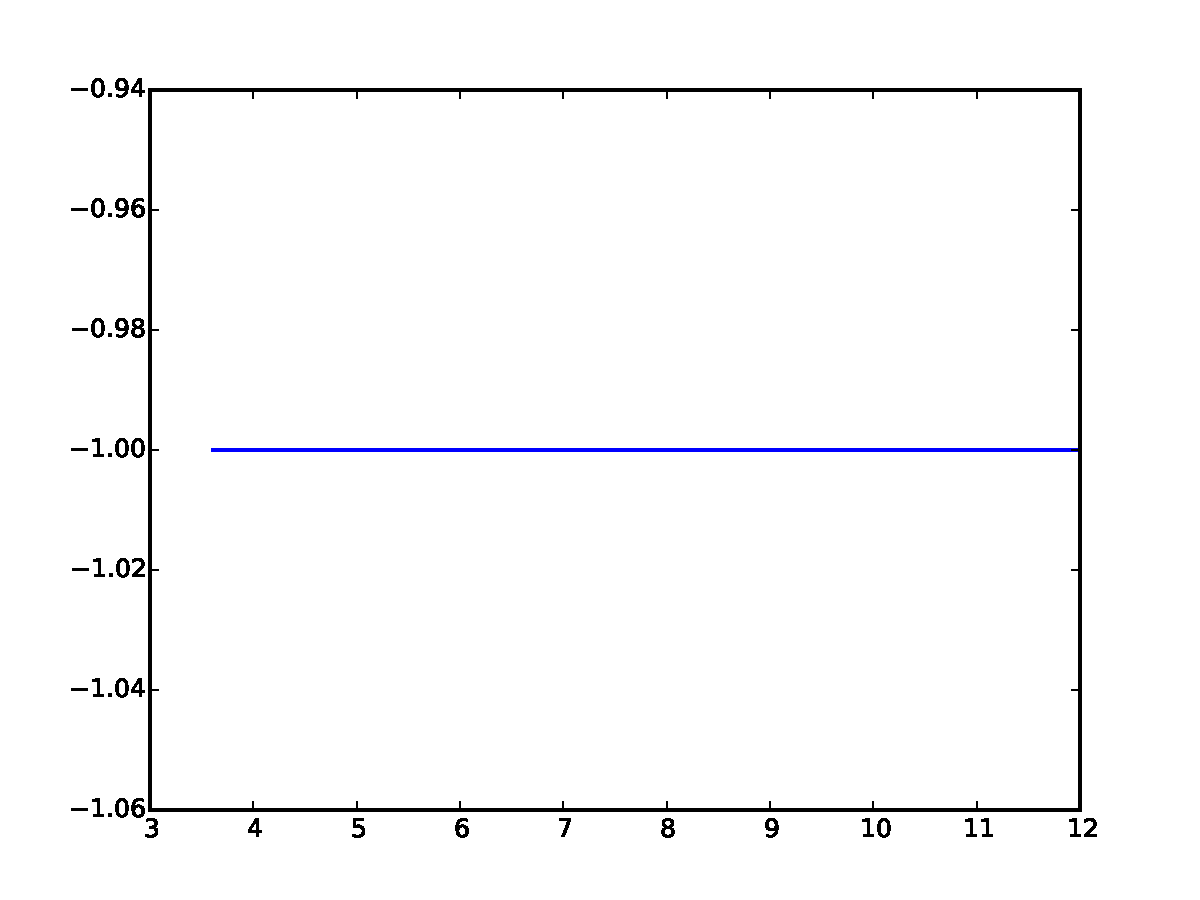
\includegraphics[width=0.97\linewidth]{bootstrap-filter/relative_tail_complex_3_1.pdf}
	\end{minipage}
	\begin{minipage}{.3\textwidth}
		\centering
		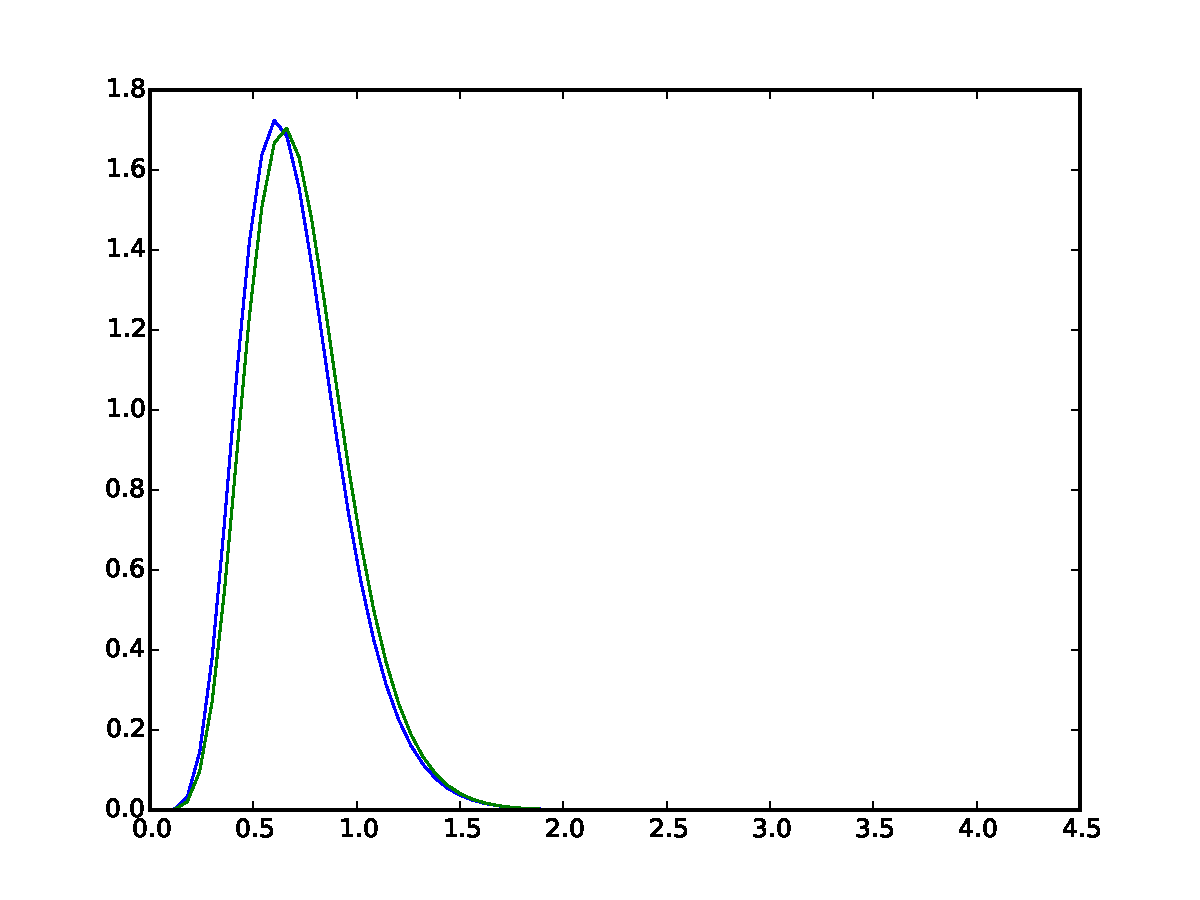
\includegraphics[width=0.97\linewidth]{bootstrap-filter/global_complex_3_9.pdf}
	\end{minipage}
	\begin{minipage}{.3\textwidth}
		\centering
		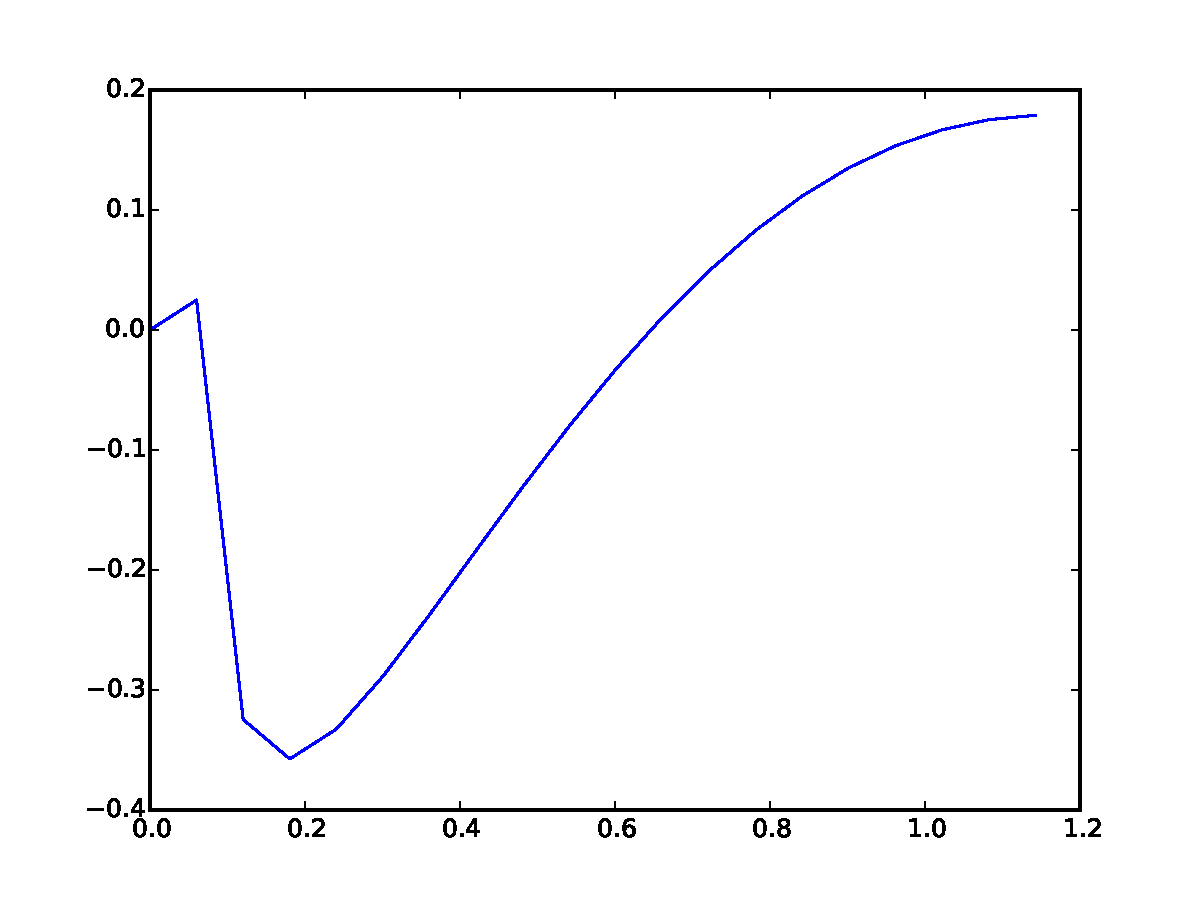
\includegraphics[width=0.97\linewidth]{bootstrap-filter/relative_beginning_complex_3_9.pdf}
	\end{minipage}
	\begin{minipage}{.3\textwidth}
		\centering
		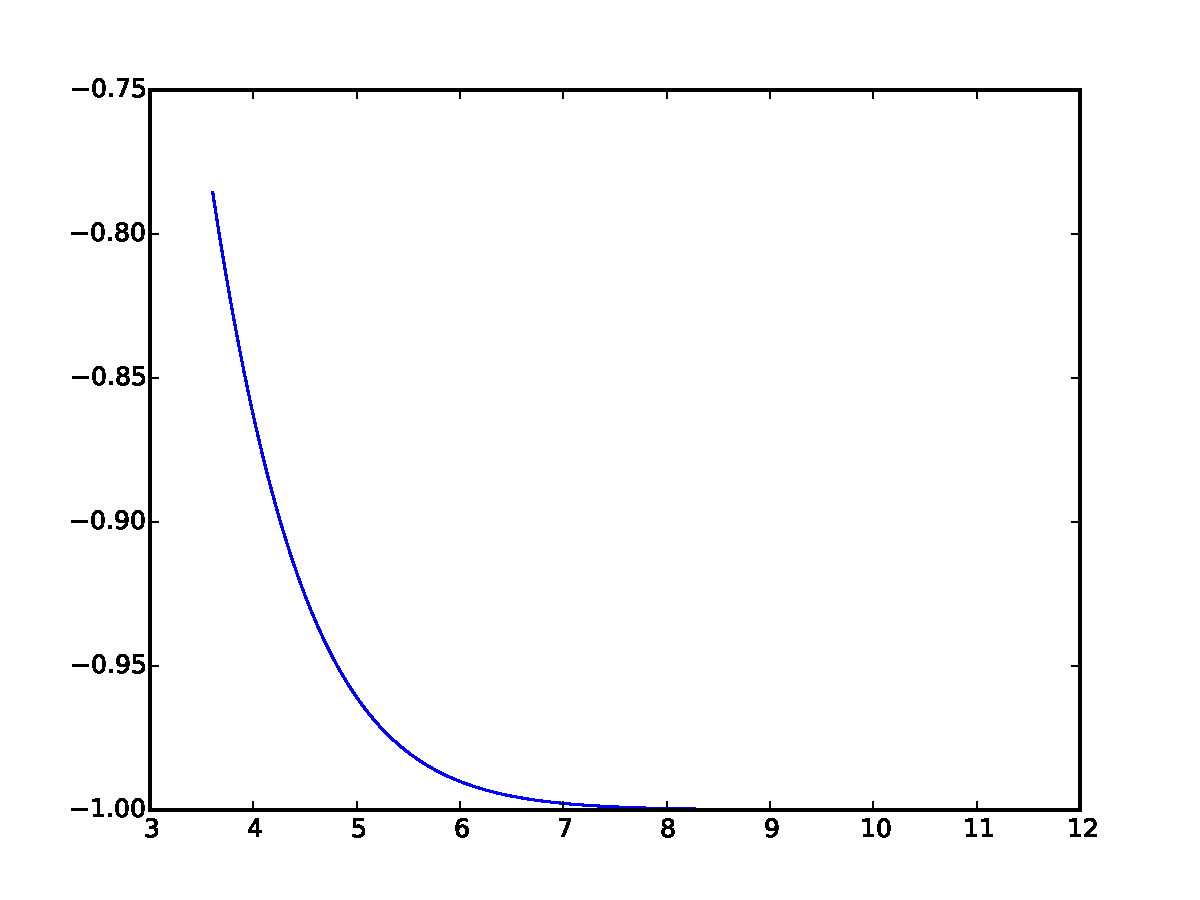
\includegraphics[width=0.97\linewidth]{bootstrap-filter/relative_tail_complex_3_9.pdf}
	\end{minipage}
	\caption{\textbf{(left)} Comparison between \textbf{(blue)} the optimal proposal density and \textbf{(green)} the gamma approximation density, \textbf{(middle)} relative error between values near 0 of the gamma approximation density and the optimal proposal density, \textbf{(right)} relative error between the right tails of the gamma approximation density and the optimal proposal density for \textbf{(first row)} $\ln(r)=1$ and $\sigma^2 = 0.3$, \textbf{(second row)} $\ln(r)=4$ and $\sigma^2 = 0.3$, \textbf{(third row)} $\ln(r)=3$ and $\sigma^2 = 0.1$, \textbf{(fourth row)} $\ln(r)=3$ and $\sigma^2 = 0.9$.}
	\label{fig:movingcomplex}
\end{figure}

\end{document}